\documentclass[twocolumn,apj,numberedappendix,twocolappendix,iop]{openjournal}
\usepackage[T1]{fontenc}

\usepackage{graphicx}	% Including figure files
\usepackage{amsmath}	% Advanced maths commands
\usepackage{newtxtext,newtxmath}    % PUT THIS ONE BACK IN IN OVERLEAF
\usepackage[dvipsnames]{xcolor}  
\usepackage[colorlinks,linkcolor=blue,citecolor=blue,urlcolor=blue ]{hyperref}
\usepackage{amssymb}	% Extra maths symbols
\usepackage{dsfont}
\usepackage{ulem}
\usepackage{soul}
\usepackage{enumitem}
\usepackage{orcidlink}
\usepackage{hyperref}

\usepackage{natbib}
\usepackage{fontawesome}
\usepackage{lineno}
\usepackage{macros}
\usepackage{float}
\usepackage{multirow}

\begin{document}

\title{Halo Assembly Bias in Excursion Set-Based Subhalo Abundance Measurements}

\shorttitle{Halo Assembly Bias in SatGen}
\shortauthors{Monzon et al.}

\author{J. Sebastian Monzon\orcidlink{0000-0002-9986-4604}}
\author{Frank C. van den Bosch\orcidlink{0000-0003-3236-2068}}
\author{Kaustav Mitra\orcidlink{0000-0001-8073-4554}}

\affiliation{Department of Astronomy, Yale University, PO. Box 208101, New Haven, CT 06520-8101}
\jsm{Kaustav plz add your affiliation}
\email{s.monzon@yale.edu}

\begin{abstract}

\end{abstract}

\section{Introduction}
\label{sec:intro}

Halo occupation modeling has become a key method for constraining the galaxy--halo connection (see \citealt{Wechsler.Tinker.18} for a review). It uses observables such as galaxy clustering \citep[][]{Berlind.Weinberg.02, vdBosch.etal.07, Zehavi.etal.11}, galaxy--galaxy lensing \citep{Mandelbaum.etal.06, Cacciato.etal.13, Leauthaud.etal.17}, satellite kinematics \citep{More.etal.09b, Lange.etal.19a, Mitra.etal.24}, and galaxy group catalogs \citep{Weinmann.etal.06, Yang.etal.07, Tinker.etal.12} to establish a statistical link between the properties of galaxies and the dark matter halos they inhabit. In the vast majority of cases, the occupation statistics are parameterized solely as a function of halo mass. For example, the Halo Occupation Distribution \citep[HOD;][]{Berlind.etal.03, Zheng.etal.05} characterizes the probability $P(N|M)$ that a halo of mass $M$ contains $N$ galaxies (typically above a given stellar mass or luminosity), while the Conditional Luminosity Function \citep[CLF;][]{Yang.etal.03, vdBosch.etal.13}, $\Phi(L|M)\,{\rm d}L$, gives the average number of galaxies with luminosities in the range $L \pm {\rm d}L/2$ residing in a halo of mass $M$.

While these frameworks have proven highly successful at reproducing a wide range of observed summary statistics, they assume that galaxy occupation depends on halo mass alone, neglecting any dependence on halo assembly history or large-scale environment. Yet numerical simulations of structure formation have shown that dark matter halos of fixed mass exhibit different clustering strengths depending on their assembly history, concentration, spin, and shape \citep{Gao.etal.05, Wechsler.etal.06, Gao.White.07, Dalal.etal.08, Giocoli.etal.10, Faltenbacher.White.10, Mao.etal.18, Paranjape.etal.18}. This phenomenon is commonly referred to as \textit{halo} assembly bias. If galaxy occupation statistics also depend on these secondary halo properties at fixed halo mass, the resulting effect is known as \textit{galaxy} assembly bias (GAB) \citep[][]{Zentner.etal.14}.

Considerable effort has been devoted to searching for evidence of GAB \citep{Yang.etal.06, Berlind.etal.06, Tinker.etal.08, Hearin.etal.16, Zu.Mandelbaum.18}, yet establishing its existence and magnitude remains challenging. Doing so requires correlating galaxy observables with secondary halo properties that are difficult to constrain observationally \citep{Miyatake.etal.16, Zu.etal.17, Lin.etal.16, Sunayama.More.19}, while controlling for halo mass, which is itself uncertain \citep{Campbell.etal.15, Old.etal.15}. Understanding and quantifying GAB is nevertheless important for two main reasons. First, any correlation between galaxy observables and secondary halo properties provides valuable insight into the physical processes governing galaxy formation and evolution. Such correlations encode information about the interplay between halo growth, gas accretion, star formation, and merger rates \citep{Somerville.etal.15, Behroozi.etal.19}. Second, any inference based on halo occupation models that ignore dependencies on secondary halo properties may be systematically biased \citep{Zentner.etal.14, Hearin.etal.15}. This is particularly worrisome in the context of precision cosmology, where percent-level constraints on cosmological parameters increasingly rely on accurate forward models of the galaxy--halo connection \citep{Weinberg.etal.13, Hearin.etal.16, Mitra.vdBosch.25}.

In the standard halo model, galaxy clustering separates into a one-halo term, from galaxy pairs within the same halo, and a two-halo term, from pairs in distinct halos \citep{Seljak.00, Cooray.Sheth.02, vdBosch.etal.13}. The one-halo term, which dominates on scales $\lesssim 1\,h^{-1}{\rm Mpc}$, is set by the number of satellites per halo, and is therefore directly sensitive to any dependence of satellite (and hence subhalo) abundance on host assembly history \citep{Zentner.etal.14, Hearin.etal.16}. Such a dependence is well established: host halos that form earlier host fewer surviving subhalos, both in semi-analytic models \citep{Zentner.etal.05, vdBosch.etal.05a, Jiang.vdBosch.17} and numerical simulations \citep[][]{Zhu.etal.06, Giocoli.etal.08, Ishiyama.etal.09}. This is in part because earlier-forming halos are more concentrated \citep[][]{Wechsler.etal.02, Zhao.etal.09, Mao.etal.15}. The physical origin of these trends is intuitive. More concentrated hosts exert stronger tides and are therefore more efficient at disrupting their substructure \citep{vdBosch.etal.18a}. Furthermore, the earlier a subhalo is accreted, the longer it is exposed to these tides, and the more likely it is to be stripped below a fixed mass threshold \citep{Jiang.vdBosch.16, Mao.etal.15}. Throughout this paper, we refer to these correlations between subhalo abundance and host halo assembly history as signals of \textit{assembly bias}, although they are not themselves clustering measurements.

% As discussed in \citet{Giocoli.etal.08} and \citet{Jiang.vdBosch.16}, the dependence on formation redshift owes to the fact that the unevolved subhalo mass function (i.e., the mass function of subhalos at accretion) is universal. Statistically speaking, all halos assemble from the same mass building blocks, and halos that assemble earlier simply accrete these building blocks earlier. The formation time, $\zfive$, provides a direct measure of when the host assembled, while the present-day concentration, $\cvir$, provides a related measure of the structural imprint of that assembly history. Comparing $\zfive$ and $\cvir$ allows us to isolate what components of the \SatGen\ model might be responsible for inconsistencies in the measured assembly bias signals.

Semi-analytic models offer an efficient means of studying the connection between subhalo abundance and host halo assembly. One such model is the SATellite Galaxy GENerator (\SatGen; \citealp{Jiang.etal.21}), which combines merger trees generated using extended Press--Schechter (EPS) theory \citep{Parkinson.etal.08} with analytical prescriptions for the orbital evolution, tidal stripping, and disruption of accreted subhalos. This approach enables the generation of large ensembles of merger trees and their associated subhalo populations at a fraction of the computational cost of $N$-body simulations, while reproducing their merger-tree statistics \citep{Jiang.vdBosch.14, vdBosch.etal.14} and subhalo populations \citep{Jiang.etal.21} with high accuracy. Consequently, EPS-based methods remain widely used for studying halo assembly and substructure, even in the era of high-resolution cosmological simulations (e.g., \citealp{Folsom.etal.2023, Nadler.etal.23b, Danieli.etal.23, Monzon.etal.24, Dropulic.etal.25, Li.etal.26, Monzon.etal.26}). Nevertheless, the simplifying assumptions underlying the \SatGen\ model introduce two potential limitations.

First, the EPS-based merger trees used by the \SatGen\ model do not explicitly account for the influence of large-scale environment on halo assembly. In particular, the Markovian nature of the underlying formalism implies that halo assembly histories are statistically independent of environment at fixed halo mass \citep{Zentner.07, Ma.etal.11, Zhang.etal.14}. This contrasts with $N$-body simulations, where merger rates, progenitor mass functions, and diffuse accretion rates have been shown to depend on environment, even at fixed halo mass \citep{Fakhouri.Ma.09, Fakhouri.Ma.10}. In dense environments, for example, the tidal field of neighboring massive halos can stall the mass accretion of a halo, and with it the accretion of new subhalos \citep{Dalal.etal.08, Hahn.etal.09}. Because environment can shape both when a halo assembles and which subhalos it accretes, it may strengthen the correlation between the two beyond what EPS trees can reproduce. 

Second, the \SatGen\ model treats the host halo assembly history separately from the dynamical evolution of its subhalos. In practice, the merger tree is generated first, fixing the host halo's mass accretion history (MAH). The host concentration is then assigned as a deterministic function of this history \citep{Zhao.etal.09}, with no additional scatter at fixed assembly history. The subsequent orbital evolution of accreted subhalos is then calculated within this predetermined host halo potential. Consequently, the accretion and evolution of substructure cannot modify the host's concentration or density profile, and any correlation between subhalo abundance and concentration in the \SatGen\ model must arise entirely through their common dependence on the MAH. This differs from $N$-body simulations, where host halos and their substructure evolve self-consistently, allowing accreted subhalos to perturb the host potential and alter its density distribution. Moreover, concentrations in simulations are measured from the particle distribution of the host, which includes its bound substructure \citep{Behroozi.etal.13a, Prada.etal.12, Wang.etal.20, Fielder.etal.20, Mezini.etal.23}, so that subhalo abundance directly affects the measured concentration. This is in contrast with the \SatGen\ framework that models all host halo densities analytically as smooth profiles.

In this paper, we investigate the extent to which these limitations affect the correlations between subhalo abundance and host halo assembly history. By comparing predictions from the \SatGen\ model against two cosmological $N$-body simulations, Bolshoi--Planck and VSMDPL, we assess its ability to reproduce the strength of these correlations and explore the physical origins of any discrepancies. Although subhalo abundance is not itself a direct observable, understanding its dependence on assembly history is an essential step toward measuring GAB in satellite populations. This paper is organized as follows: Section~\ref{sec:methods} describes our semi-analytic framework and the dark-matter-only (DMO) simulations used for comparison. Section~\ref{sec:results} presents our fiducial results: although the \SatGen\ model reproduces the sign and halo-mass dependence of the correlations between subhalo abundance and both formation redshift and concentration, it underestimates their strength by [XX] relative to the simulations. Section~\ref{sec:discussion} identifies the origin of this discrepancy, which we trace to [YY], and discusses possible improvements to the semi-analytic framework. \jsm{update this roadmap: Section \ref{sec:tests} now tests the concentration channel (relaxed hosts, a single mass bin, the \cite{Ludlow.etal.16} model and measured concentrations) and Section \ref{sec:discussion} discusses the results.} Finally, Section~\ref{sec:conclusions} summarizes our results.

\section{Methods}
\label{sec:methods}

\subsection{SatGen}
\label{sec:satgen}

Our analysis employs the \SatGen\ model, a state-of-the-art semi-analytic model that generates statistical samples of satellite galaxy populations. The \SatGen\ model \citep{Jiang.etal.21} constructs merger trees for host halos using the EPS-based method of \citet{Parkinson.etal.08}. These merger trees describe the infall mass and accretion time of all progenitor halos that coalesce to form the final host halo. They are constructed under the assumption of a Markovian random walk and are therefore agnostic about the surrounding cosmic environment. Each host halo is assigned an NFW profile whose concentration is set using the model of \citet{Zhao.etal.09}, in which $\cvir$ is determined by the cosmic density when the main progenitor first reaches 4\% of its present-day mass. For each host we also record the half-mass formation redshift, $\zfive$, at which the main progenitor first reaches half of its present-day mass.

Once a merger tree is constructed, the \SatGen\ model evolves subhalos by integrating their orbits within this analytic, spherically symmetric host halo potential that evolves with time. Subhalo positions and velocities are determined from point particle orbit integration. These orbits inform semi-analytic prescriptions \citep{vdBosch.Jiang.16, Jiang.vdBosch.17, Green.vdBosch.19} that model tidal stripping, tidal heating and dynamical friction. The \SatGen\ model resolves substructure hierarchically, where first-order subhalos are those that were accreted directly onto the host, second-order subhalos (``sub-subhalos'') are those that were accreted onto first-order subhalos, and so on for subhalos of order $n$. Each subhalo's orbit is integrated within its immediate (order $n-1$) parent. 

To control for halo mass, we generate samples of 1,000\footnote{As shown in Appendix D of \citealt{Monzon.etal.24}, this is sufficient for probing the effects of halo-to-halo variance.} unique merger trees for 8 different values of host halo mass. In what follows, we refer to these samples using the shorthand notation $\mathbb{S}_m$, where $m \equiv \log(\Mvir/\Msunh) \in \{12.6, 12.8, \dots, 13.8, 14.0\}$. Each merger tree traces the evolution of all its branches down to the same minimum progenitor or ``leaf'' mass of $10^{9}\,\Msunh$, which is roughly an order of magnitude above the theoretical hydrogen cooling limit \citep{Greif.etal.08}. This corresponds to a mass resolution that ranges from $10^{-3.6}\,\Mvir$ for $\mathbb{S}_{12.6}$ to $10^{-5}\,\Mvir$ for $\mathbb{S}_{14.0}$. These 8 individual samples provide a clean baseline in which all variation arises from differences in assembly history and the stochastic orbits of accreted subhalos, while a comparison among the 8 different samples allows us to test for halo mass dependencies. Unless stated otherwise, all merger trees adopt a Planck-consistent\footnote{We have verified that these minor differences in cosmology compared to the MultiDark suite do not significantly impact our results regarding the strength of the assembly bias signal.} $\Lambda$CDM cosmology with $\Omega_{M}=0.3$, $\Omega_{B}=0.0465$, $\Omega_{\Lambda}=0.7$, $\sigma_8 = 0.8$, $n_s=1.0$, and $H_0=70\,\mathrm{km\,s^{-1}\,Mpc^{-1}}$.

\subsection{DMO Simulations}
\label{sec:sims}

We compare the \SatGen\ model with two different high-resolution cosmological $N$-body simulations taken from the MultiDark suite \citep{Klypin.etal.11, Riebe.etal.13, Klypin.etal.16, RodriguezPuebla.etal.16}. These dark-matter-only (DMO) simulations model structure formation in a Planck-consistent $\Lambda$CDM cosmology with parameters $\Omega_{M}=0.307$, $\Omega_{B}=0.048$, $\Omega_{\Lambda}=0.693$, $\sigma_8 = 0.823$, $n_s=0.96$, and $H_0=67.8\,\mathrm{km\,s^{-1}\,Mpc^{-1}}$. In particular, we use both the Bolshoi--Planck (hereafter BolshoiP) simulation and the Very Small MultiDark Planck simulation (hereafter VSMDPL). 
%
\begin{table}[htbp]
\centering
    \begin{tabular}{c|c|c|c}
    \hline
    \hline
    Simulation & $L_{\rm box}$ [$\mpch$] & $m_{\rm p}$ [$\Msunh$] & $\epsilon$ [$\kpch$] \\
    \hline
    BolshoiP & 250 & $1.55 \times 10^{8}$ & 1.0  \\
    VSMDPL   & 160 & $6.20 \times 10^{6}$ & 2.0 \\
    \hline
    \end{tabular}
    \caption{A summary of the MultiDark simulations used in this analysis. From left to right the columns correspond to simulation name, box size, particle mass, and softening length. Further details regarding both simulations can be found in \cite{Klypin.etal.11, Riebe.etal.13, Klypin.etal.16, RodriguezPuebla.etal.16}.}
    \label{tab:sims}
\end{table}

BolshoiP follows the evolution of $2048^3$ dark matter particles using the Adaptive Refinement Tree (ART) gravity solver \citep{Kravtsov.etal.97}. The simulation has a box size of $250 \mpch$ and a particle mass of $1.55\times10^{8}\,\Msunh$ (see Table~\ref{tab:sims}). VSMDPL complements BolshoiP by providing significantly higher mass resolution over a smaller cosmological volume \citep{Klypin.etal.16, RodriguezPuebla.etal.16, Behroozi.etal.20}. It follows $3840^3$ particles using an optimized version of the \texttt{GADGET-2} gravity solver \citep{Springel.05} with a box size of $160 \mpch$ and a particle mass of $6.2\times10^{6}\,\Msunh$ (see Table~\ref{tab:sims}). While BolshoiP is better suited for capturing the statistics of the more massive systems, VSMDPL more reliably resolves the dynamics and evolution of lower-mass (sub)halos. In Section \ref{sec:fid_HAB}, we leverage this to demonstrate that the assembly bias signals we measure in DMO simulations are stable across more than an order of magnitude in subhalo mass resolution. 

We use the publicly available\footnote{https://www.cosmosim.org} halo catalogs and merger trees obtained using the phase-space halo finder \texttt{ROCKSTAR} \citep{Behroozi.etal.13a, Behroozi.etal.13b}, which employs adaptive, hierarchical refinement of friends-of-friends groups in six phase-space dimensions and one time dimension. As demonstrated in \citet{Knebe.etal.11, Knebe.etal.13} and \citet{Onions.etal.12}, this results in robust tracking of (sub)halos\footnote{Although several newer halo-finding algorithms have been developed, such as \texttt{SYMFIND} \citep{Mansfield.etal.24} and \texttt{BLOODHOUND} \citep{Kong.etal.25}, we adopt \texttt{ROCKSTAR} because it provides a consistent set of publicly available catalogs for both simulations analyzed in this study.}. For each host halo, the catalogs list the halo virial mass, defined as
%
\begin{equation}
    M_{\mathrm{vir}}=\frac{4 \pi}{3} \Delta_{\mathrm{vir}}(z) \rho_{\mathrm{m}} R_{\mathrm{vir}}^3.
    \label{eq:mvir}
\end{equation}
%
the halo concentration parameter $\cvir = \Rvir/\rs$, and the half-mass formation redshift $\zfive$. Here, $\Delta_{\mathrm{vir}}(z)$ is the redshift- and cosmology-dependent overdensity threshold derived from the spherical collapse model \citep{Bryan.Norman.98}, $\Rvir$ is the halo virial radius, and $\rs$  is the characteristic radius of an NFW profile \citep{Navarro.etal.97}. Note that the halo concentrations are inferred from the ratio of the maximum circular velocity, $V_{\rm max}$, to the virial velocity, $V_{\rm vir}$ \citep[][]{Klypin.etal.11, Prada.etal.12}, rather than from explicitly fitting the density profile.

We construct samples from BolshoiP and VSMDPL by selecting host halos within narrow mass bins centered on the discrete mass values described in Section \ref{sec:satgen}. This minimizes the impact of host halo mass-mixing, and helps ensure that variations in subhalo populations are primarily driven by assembly history. We find that a $\pm 0.1$ dex mass window provides a suitable balance between minimizing host halo mass-mixing and retaining sufficient statistics (see Appendix XXX for an exploration of wider mass bins).

\subsection{Subhalo Summary Statistics}
\label{sec:counts}

By virtue of the \texttt{ROCKSTAR} halo finder, dark matter subhalos are defined as self-gravitating overdensities located inside the virial radius of a larger halo. This definition ignores ``splashback'' (or ``backsplash'') subhalos which, despite still being gravitationally bound, do not currently live within their host halo's virial radius \citep{More.etal.16, Diemer.17, Mansfield.etal.17, Haggar.etal.20}. In order to allow for a meaningful comparison, we therefore apply a similar cut to the subhalo population in the \SatGen\ model and only include those subhalos that are instantaneously located within the virial radius of the host. As shown in \citet{Green.etal.21}, this removes close to 50 per cent of the entire population of surviving subhalos that have previously been accreted into the host.

For both the \SatGen\ model and the DMO simulations, we measure the number of surviving subhalos with an instantaneous mass $m_{\rm sub}$ larger than a specific minimum threshold mass $\mthresh$, as
%
\begin{equation}
\nsub = \sum_{i=1} \Theta(m_{{\rm sub},i} - \mthresh) \, \Theta(\Rvir - |\vec{r}|_i)\,.
\label{eq:Nsub}
\end{equation}
%
Here, $\Theta(x)$ is the Heaviside step function and $\vec{r}$ is the instantaneous position vector of the subhalo with respect to the center of its host halo whose virial radius is $\Rvir$. Throughout, we adopt $\mthresh = 7.75 \times 10^{10}\Msunh$ as our fiducial value, which corresponds to subhalos with at least 500 (12,500) particles in BolshoiP (VSMDPL). We also measure, for each host halo, the corresponding present-day subhalo mass \textit{fraction}, defined according to
%
\begin{equation}
    \fsub = \frac{1}{\Mvir} \sum_{i=1} \left[ m_{{\rm sub},i}\, \Theta \left(m_{{\rm sub},i} - \mthresh \right)\,\Theta(\Rvir - |\vec{r}|_i)\right].
\label{eq:fsub}
\end{equation}
%

The two summary statistics $\nsub$ and $\fsub$ are complementary in that $\nsub$ is particularly sensitive to the more abundant low-mass subhalos, whereas $\fsub$ more heavily weights the most massive subhalos. 

\begin{figure}
    \centering
    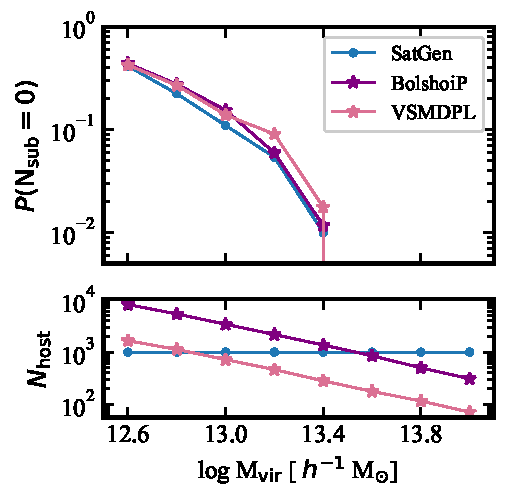
\includegraphics{figures/Nhosts.pdf}
    \caption{Top: Probability that a host halo contains no surviving subhalos, $P(\nsub = 0)$, as a function of host halo mass for the \SatGen\ model (blue), BolshoiP (purple), and VSMDPL (pink). The rise in $P(\nsub = 0)$ toward lower host masses reflects the fact that these hosts contain fewer subhalos above the fixed threshold $\mthresh$. Bottom: Number of host halos, $\Nhost$, selected within each narrow ($\pm 0.1$ dex) mass bin. While $\Nhost$ decreases with increasing $\Mvir$ in the fixed-volume simulations, the \SatGen\ model samples $\Nhost = 1000$ regardless of the mass bin.}
    \label{fig:nhosts}
\end{figure}
 
\subsection{Measuring Assembly Bias Signals}
\label{sec:correlation}

The main goal of this study is to assess how $\nsub$ and $\fsub$ are correlated, at fixed halo mass, with secondary host halo properties. The secondary properties we focus on are halo formation redshift, $\zfive$, and host halo concentration, $\cvir$. These properties are known to be strongly correlated with each other because higher-concentration halos form earlier \citep{Wechsler.etal.02} and the density profile of a halo is directly affected by its unique accretion history \citep{Lu.etal.06, Ludlow.etal.13, Lucie-Smith.etal.22}. 

We quantify the assembly bias signal between $\nsub$/$\fsub$ and $\zfive$/$\cvir$ using four Spearman rank-order correlation coefficients: $\rho_S(\nsub, \zfive)$, $\rho_S(\fsub, \zfive)$, $\rho_S(\nsub, \cvir)$ and $\rho_S(\fsub, \cvir)$. All coefficients are measured within each $\mathbb{S}_m$ mass bin, and hosts with $\nsub = 0$ are kept and share the lowest rank. For the reasons outlined in Section~\ref{sec:intro}, we expect all four coefficients to be negative \citep{Zentner.etal.05, Jiang.vdBosch.17, Mao.etal.15}. 

To account for the fact that $\zfive$ and $\cvir$ are themselves correlated, we also measure four other distinct \textit{partial} rank correlations. These partial correlations detail how much the measured correlation between two variables is a consequence of their common dependence on a third, related variable. For $X \in \{\nsub, \fsub\}$, we define
%
\begin{equation}
\rho_S(X, \cvir \,|\, \zfive) = \frac{\rho_S(X, \cvir) - \rho_S(X, \zfive)\,\rho_S(\zfive, \cvir)}{\sqrt{\left[1-\rho_S(X, \zfive)^2\right]\left[1-\rho_S(\zfive, \cvir)^2\right]}}\,,
\label{eq:partial}
\end{equation}
%
as the rank correlation between $X$ and $\cvir$ at fixed $\zfive$. If $X$ and $\cvir$ were related only through their common dependence on $\zfive$, their correlation would be the product $\rho_S(X, \zfive)\,\rho_S(\zfive, \cvir)$. The numerator therefore measures how much the measured $\rho_S(X, \cvir)$ departs from this expectation, and the denominator normalizes the result to $[-1, 1]$. A non-zero value thus indicates that $\cvir$ carries information about subhalo abundance beyond what $\zfive$ already provides. Since the fixed variable is held statistically rather than by sub-binning, the partial correlations use the full sample of hosts in each mass bin. Interchanging $\zfive$ and $\cvir$ gives $\rho_S(X, \zfive \,|\, \cvir)$, which measures how well $\zfive$ predicts $X$ at fixed $\cvir$. We refer to $\rho_S(X, \cvir \,|\, \zfive)$ as the \textit{concentration channel} and $\rho_S(X, \zfive \,|\, \cvir)$ as the \textit{formation-time channel}.

To quantify the statistical significance of these correlation coefficients, we estimate uncertainties on $\rho_S$ using a jackknife resampling procedure. For each host halo sample, we first compute the correlation coefficient using the full number of hosts per $\Mvir$ interval (see Figure~\ref{fig:nhosts}). We then randomly partition each sample into $N_{\rm jk} = 10$ subsets and iteratively recompute $\rho_S$ while omitting one subset at a time. This produces distributions from which we estimate the variance using the standard jackknife estimator
%
\begin{equation}
\mathrm{Var}(\rho_S) = \frac{N_{\rm jk}-1}{N_{\rm jk}} \sum_{i=1}^{N_{\rm jk}} \left( \rho_i - \bar{\rho} \right)^2,
\end{equation}
%
where $\rho_i$ is the correlation coefficient computed from the $i$-th jackknife realization and $\bar{\rho}$ is the mean of the jackknife estimates across all realizations. We apply the same procedure to the partial correlations.

\section{Results}
\label{sec:results}

\subsection{First-Order Comparisons}
\label{sec:scaling}

\begin{figure*}
    \centering
    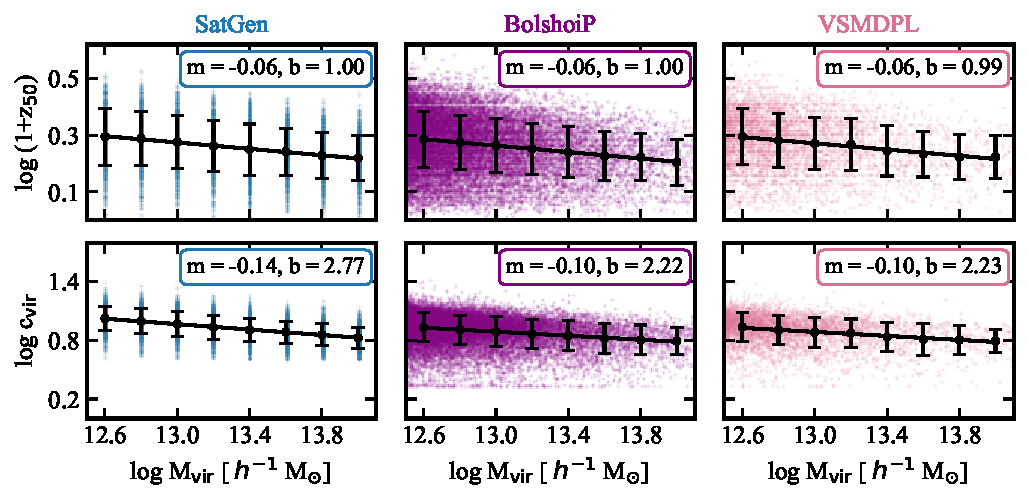
\includegraphics{figures/scaling_relations.pdf}
    \caption{Several best-fit scaling relations for the \SatGen\ model (blue), BolshoiP (purple) and VSMDPL (pink). The top row shows the half-mass formation redshift ($\zfive$) and the bottom row shows the host halo concentration ($\cvir$). Colored points represent individual host halos, while black error bars show the mean and standard deviation. Lines are fit to these means, with slopes ($m$) and intercepts ($b$) indicated. Notice the overall consistency across all three models despite minor differences in assumed cosmologies, simulation volume sizes, and subhalo resolutions.}
    \label{fig:scaling}
\end{figure*}

Before comparing any second-order assembly bias measurements, it is important to confirm that the first-order scaling relations with $\Mvir$ are consistent across the models. This is because any substantial offsets in the host halo properties would make it difficult to interpret differences in assembly bias signal across the models. Figures \ref{fig:nhosts}, \ref{fig:scaling} and \ref{fig:SHMF} show how the \SatGen\ model compares to the MultiDark suite. Throughout this section, the \SatGen\ model is colored in blue, BolshoiP is colored in purple, and VSMDPL in pink.

The top panel of Figure~\ref{fig:nhosts} shows the fraction of systems that contain no surviving subhalos according to our fiducial mass threshold of $\mthresh = 7.75 \times 10^{10}\Msunh$. This metric, along with the full subhalo mass functions (see Figure \ref{fig:SHMF}), is an important check on subhalo abundance. As expected, this probability increases towards lower host halo masses, which host fewer subhalos above our fixed threshold of $\mthresh$. Among the mass intervals considered, only the $\mathbb{S}_{12.6}$ sample has $P(\nsub = 0)$ $\gtrsim 0.4$, while all host samples above $\Mvir = 10^{13.4} \Msunh$ have essentially no empty hosts. Compared to both simulations, the \SatGen\ model underpredicts $P(\nsub = 0)$ by at most $\Delta P \approx 0.05$ in the most discrepant mass bins. This slight excess of subhalos just above $\mthresh$ is also seen in Figure~\ref{fig:SHMF}. 

The bottom panel of Figure~\ref{fig:nhosts} shows the number of host halos, $\Nhost$, selected within the $\pm 0.1$ dex mass bins. In the MultiDark suite, $\Nhost$ decreases with increasing $\Mvir$ as a consequence of the finite simulation volumes. In contrast, the \SatGen\ model is sampled such that $\Nhost$ is independent of host halo mass. As we show later in Section \jsm{XXX}, despite the substantial variation in sample size across mass bins and models, our measurements of assembly bias are largely insensitive to $\Nhost$.

Figure~\ref{fig:scaling} shows scaling relations for the two host halo properties related to assembly history. The top row shows $\zfive$ and the bottom row shows $\cvir$. From left to right, the three columns show the \SatGen\ model, BolshoiP and VSMDPL. Here each colored point corresponds to an individual host halo, while the black error bars show the mean and standard deviation across the $\pm 0.1$ bins in $\Mvir$. The solid black lines are simple linear fits to these means and their associated slopes ($m$) and intercepts ($b$) are shown at the top of each panel for reference.

The top row of Figure \ref{fig:scaling} shows that more massive halos tend to assemble 50\% of their present-day mass later. This is because structure formation in $\Lambda$CDM proceeds hierarchically, where smaller progenitor halos collapse first and subsequently merge to form progressively larger systems. By design, the \SatGen\ model reproduces the negative relation between $\Mvir$ and $\zfive$ seen in the simulations. The bottom row of Figure \ref{fig:scaling} shows that more massive halos also tend to be less centrally concentrated. This is mainly due to the connection between halo concentration and formation time. Halos that assemble earlier did so when the mean density of the Universe was higher which produces denser inner regions and therefore larger concentrations. The \SatGen\ prescription for assigning host halo concentrations is set by the \cite{Zhao.etal.09} model which was calibrated on a variety of $N$-body simulations such that the same set of model parameters works well for different cosmologies and for halos of different masses across cosmic time. Similarly, the \SatGen\ model captures  the negative relation between $\Mvir$ and $\cvir$ as seen in the simulations. However, the concentrations in the \SatGen\ model are systematically higher than in the simulations, by $\sim$0.09 dex in the $\mathbb{S}_{12.6}$ sample decreasing to $\sim$0.03 dex in the $\mathbb{S}_{14.0}$ sample, which is why the fitted slope is somewhat steeper ($m = -0.14$ compared to $m = -0.10$). In contrast, the $\zfive$ relations agree to within $\sim$0.01 dex in every mass sample. We return to the concentrations in the \SatGen\ model, and to the extended tail towards low $\cvir$ seen in the simulations, in Section~\ref{sec:fid}.

The \SatGen\ model has been demonstrated to accurately reproduce the average SHMFs measured in DMO simulations across several orders of magnitude in $\Mvir$ \citep[e.g.][]{vdBosch.etal.05a, Jiang.vdBosch.16, vdBosch.etal.16, Green.vdBosch.19}. Figure \ref{fig:SHMF} shows how our fiducial model compares to the MultiDark suite to highlight any discrepancies in the $\nsub/\fsub$ distributions we use to measure assembly bias signals. Here each panel corresponds to a different host halo mass sample and the markers show the average number of subhalos per host across 19 mass bins from $7.75 \times 10^{10} \Msunh$ to $1.0\times 10^{14} \Msunh$. In the SHMF panels, the blue shaded regions correspond to the halo-to-halo variance measured in the \SatGen\ model. Beneath each SHMF, we show the difference $\Delta \langle \nsub \rangle = \langle \nsub \rangle_{\rm sim} - \langle \nsub \rangle_{\rm SatGen}$ in each bin, so that negative values indicate an excess of subhalos in the \SatGen\ model. The SHMFs agree well above $\sim 2 \times 10^{11} \Msunh$, but the \SatGen\ model produces $\sim$10\% more subhalos just above $\mthresh$ in every mass sample. This means that $\nsub$, which is dominated by the low-mass end of the SHMF, is systematically higher in the \SatGen\ model by $\sim$5--10\%, while $\fsub$, which is weighted towards the most massive subhalos, is largely unaffected.

\begin{figure*}
    \centering
     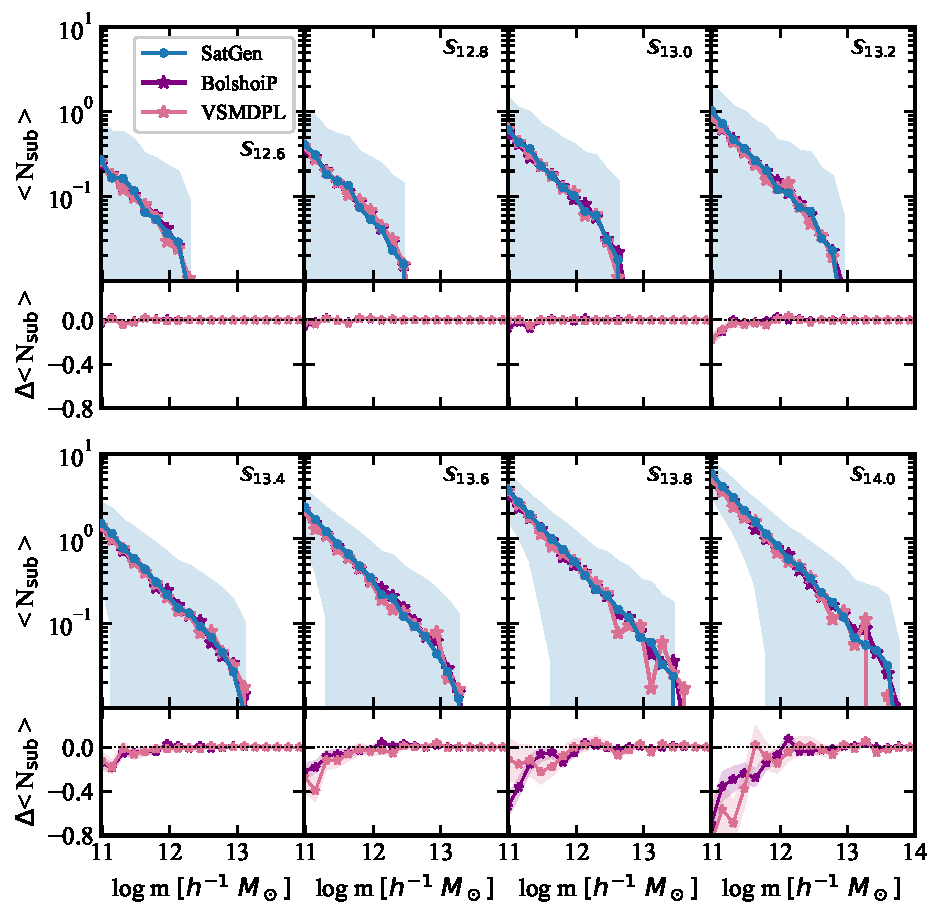
\includegraphics{figures/SHMF_all.pdf}
    \caption{A comparison of the present-day subhalo mass function (SHMF) of all three models. As before, the \SatGen\ model is shown in blue, BolshoiP in purple, and VSMDPL in pink. Each panel corresponds to a different host halo mass sample as indicated. All SHMFs have been computed with respect to the same 19 bins in subhalo mass, from our fiducial minimum mass threshold $7.75 \times 10^{10} \Msunh$ to $1.0 \times 10^{14} \Msunh$. Each point represents the average number of subhalos per host in that bin, averaged over all hosts in the sample including those with no surviving subhalos. The shaded blue region corresponds to the standard deviation in $\nsub$ per bin measured in the \SatGen\ model. Beneath each SHMF panel, we show the difference $\langle \nsub \rangle_{\rm sim} - \langle \nsub \rangle_{\rm SatGen}$ in each subhalo mass bin for BolshoiP and VSMDPL, with shaded regions marking the $1\sigma$ standard error. Negative values indicate that the \SatGen\ model predicts more subhalos than the simulations. Notice the good correspondence between all three models across the majority of mass bins.}
    \label{fig:SHMF}
\end{figure*}

Figure \ref{fig:SHMF} shows that, despite the fact that host halo mass-mixing is absent in our EPS-based merger trees (see Section \ref{sec:satgen}), the correspondence across all three models is good. In fact, the shape of the SHMF and its scaling with $\Mvir$ are reproduced in every mass sample. Often SHMFs are plotted in normalized units such that they can be fit by a power law of the form $\rm{d}N / \rm{d}\log (m/M) = A (m/M)^{-B}$ \citep{vdBosch.Jiang.16}. Though not shown explicitly, we find $B \approx 0.88$ in the \SatGen\ model which is consistent with \cite{Boylan-Kolchin.etal.10} and \cite{Green.etal.21}. 

Overall, Figures \ref{fig:nhosts}, \ref{fig:scaling} and \ref{fig:SHMF} demonstrate that despite minor differences in assumed cosmologies, simulation volume sizes, and particle resolutions, all three models are in good agreement in terms of the dominant physical processes governing subhalo populations. More precisely, the \SatGen\ model reproduces the $\zfive$--$\Mvir$ relation, the shape of the SHMF, and the trend of $P(\nsub = 0)$ with $\Mvir$. That being said, it also produces $\sim$10\% more subhalos just above $\mthresh$ and host concentrations that are higher by $\lesssim 0.1$ dex at fixed halo mass relative to the simulations. Importantly, because our assembly bias statistics are rank-order correlations measured within narrow bins of $\Mvir$, an offset that shifts all hosts in a bin by a similar amount leaves their ranks essentially unchanged. Any difference in assembly bias signal must instead reflect a difference in how assembly history and subhalo populations co-vary at fixed halo mass.

\subsection{Assembly Bias Signals}
\label{sec:fid_HAB}

\begin{figure*}
   \centering
    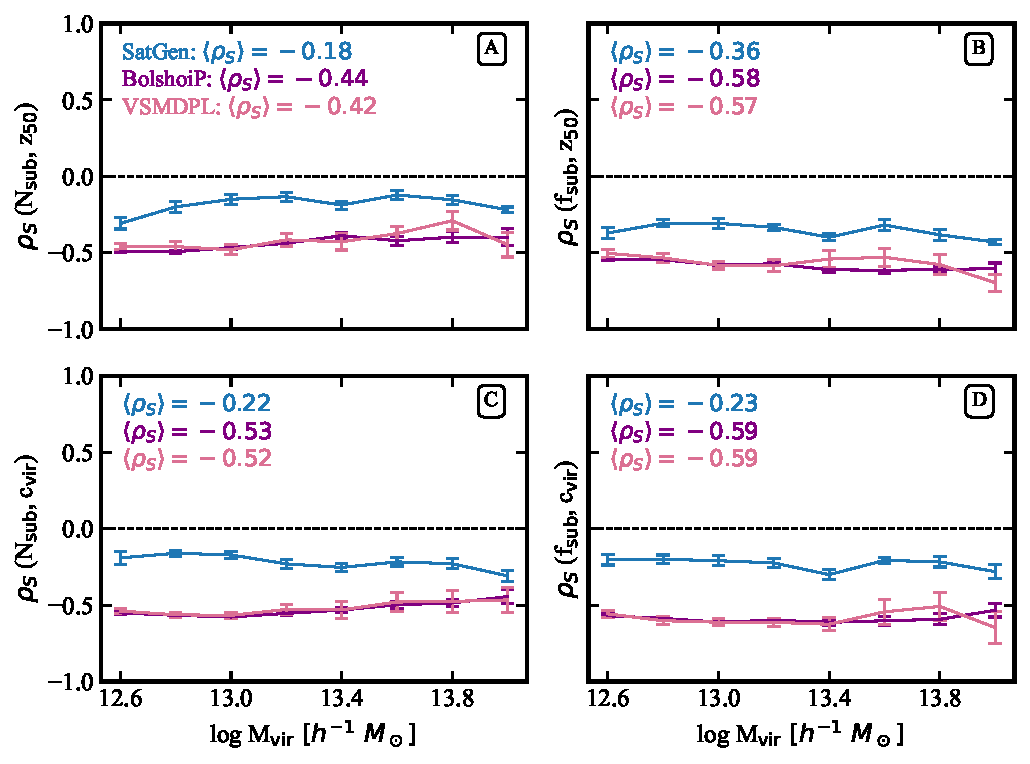
\includegraphics{figures/corr_comp.pdf}
   \caption{Assembly bias signal as a function of host halo mass for the \SatGen\ model (in blue), BolshoiP (in purple), and VSMDPL (in pink). All panels show rank-order correlation coefficients measured with the error bars corresponding to the jackknife uncertainties described in Section \ref{sec:correlation}. We show $\rho_S(\nsub, \zfive)$ in panel A, $\rho_S(\fsub, \zfive)$ in panel B, $\rho_S(\nsub, \cvir)$ in panel C, and finally $\rho_S(\fsub, \cvir)$ in panel D. The mass-averaged correlation strengths are shown in the top left corner of every panel.}
   \label{fig:correlations}
\end{figure*}

We now compare the measured assembly bias signals across all three models. Figure \ref{fig:correlations} shows $\rho_S(\nsub, \zfive)$ in panel A, $\rho_S(\fsub, \zfive)$ in panel B, $\rho_S(\nsub, \cvir)$ in panel C, and finally $\rho_S(\fsub, \cvir)$ in panel D all as a function of $\Mvir$. The error bars are the result of the jackknife analysis (see Section \ref{sec:correlation}) and the $\rho_S = 0$ line is shown for reference. Finally, to facilitate comparisons, the mass-averaged correlation strengths are printed in the top left of every panel.

All three models produce assembly bias signals that do not depend strongly on $\Mvir$. This is because though the formation times, concentrations (Figure \ref{fig:scaling}) and the normalization of the SHMF (Figure \ref{fig:SHMF}) all change with $\Mvir$, the rank-order correlations measured within our narrow mass bins do not scale with these overall shifts. Note also that regardless of the specific assembly history statistic used, $|\rho_S| \lesssim 0.6$. Both the lack of a clear mass dependence and the range of magnitudes in the correlation coefficients are consistent with results presented in \jsm{XXX}

Although the \SatGen\ model correctly predicts the sign of all correlation coefficients, it produces assembly bias signals that are weaker than in the MultiDark suite. This is not a numerical artifact in the simulations since BolshoiP and VSMDPL produce assembly bias signals that are remarkably similar despite differences in mass resolution. The discrepancy between the \SatGen\ model and the simulations is most prominent when the assembly bias signal is measured with respect to $\cvir$ but across all four statistics, we find $\Delta \rho_S \approx 0.28$. 

\begin{figure*}
   \centering
    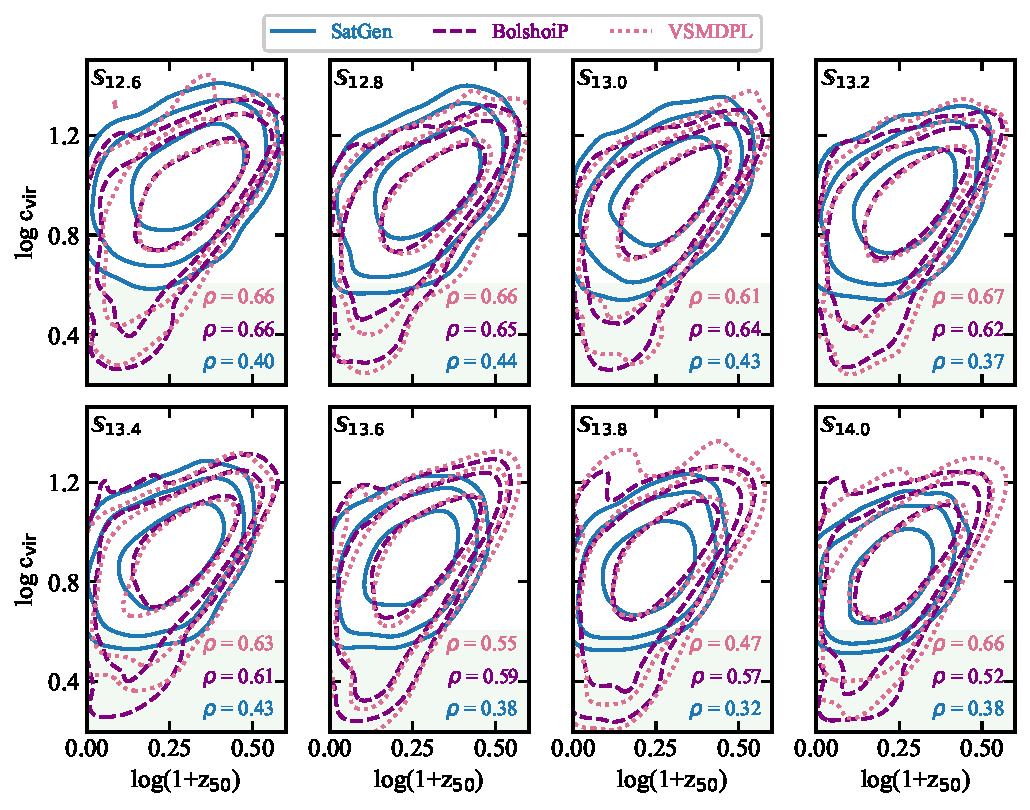
\includegraphics{figures/z50_cvir.pdf}
   \caption{The PDFs of $\zfive \times \cvir$ of the three models. As before, the models are distinguished by color as indicated by the legend and for clarity they were given different linestyles. The top left corner of every panel indicates the mass sample plotted while the text in the bottom right corner shows the $\rho_S(\zfive, \cvir)$ correlation coefficients. Finally, the light shaded region marks $\cvir < 4$, below which the concentrations in the \SatGen\ model never fall (see Section \ref{sec:fid}). Notice that as we go from lower to higher host halo masses, the distributions shift slightly downward and to the left. While the \SatGen\ model is roughly consistent with the simulations, it fails to reproduce the $\rho_S(\zfive, \cvir)$ correlation strength in all mass samples.}
   \label{fig:z50_cvir}
\end{figure*}

Although Figure \ref{fig:scaling} shows good correspondence across the models, it is also important to investigate the shapes of the distributions. Figure \ref{fig:z50_cvir} shows the PDFs of $\zfive \times \cvir$ distributions. Each panel shows a different mass sample as denoted in the upper left corner. The light shaded region marks $\cvir < 4$, below which the concentrations in the \SatGen\ model never fall (see Section \ref{sec:fid}), while the text in the lower right corner gives the rank-order correlation coefficient between half-mass formation redshift and present-day concentration $\rho_S(\zfive, \cvir)$. Though not a signal of assembly bias, this correlation coefficient (along with the extent of the $\zfive$ and $\cvir$ distributions) is also an important metric on which to compare the models.

As shown in Figure \ref{fig:z50_cvir}, although the overall correspondence in terms of the 1, 2 \& 3 $\sigma$ confidence intervals is good, the \SatGen\ model not only fails to produce the extended tail towards low $\cvir$, but also results in a weaker correlation between the MAHs and present-day halo concentrations. Averaging across all host halo mass samples we find $\langle \rho_S \rangle \approx 0.39$ in the \SatGen\ model, while $\langle \rho_S \rangle \approx 0.61$ in the MultiDark suite.  

\begin{figure*}
   \centering
   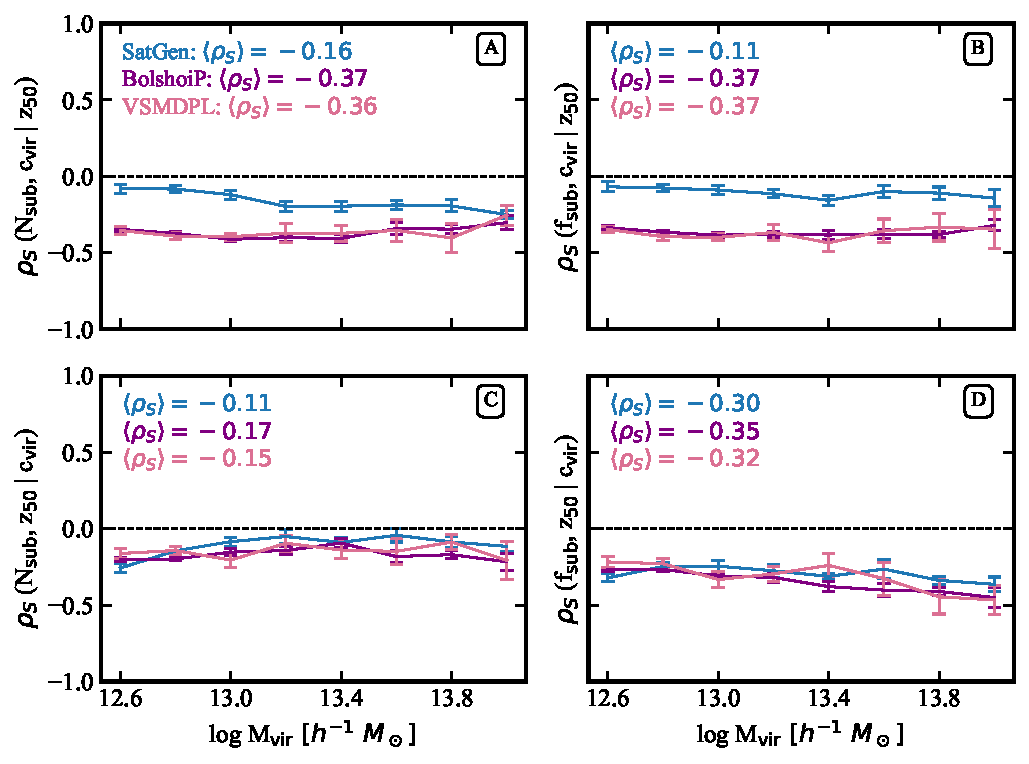
\includegraphics{figures/partial_corr.pdf}
   \caption{Partial rank-order correlations (Equation \ref{eq:partial}) as a function of host halo mass for the \SatGen\ model (blue), BolshoiP (purple) and VSMDPL (pink). The top row shows the ``concentration channel'', the correlation of $\nsub$ (panel A) and $\fsub$ (panel B) with $\cvir$ at fixed $\zfive$. The bottom row shows the ``formation-time channel'', the correlation of $\nsub$ (panel C) and $\fsub$ (panel D) with $\zfive$ at fixed $\cvir$. Error bars are jackknife uncertainties and the mass-averaged values are given in the top left of each panel. Notice how the \SatGen\ model closely matches the simulations in the formation-time channel but produces a much weaker correlation coefficient in the concentration channel.}
   \label{fig:partial}
\end{figure*}

As discussed above in Section \ref{sec:correlation}, its unclear how much of the assembly bias signals in Figure \ref{fig:correlations} are due to the fact that $\zfive$ and $\cvir$ are themselves correlated. To isolate these effects, Figure \ref{fig:partial} shows the partial correlations defined in Equation \ref{eq:partial}, using the same samples, mass bins and jackknife uncertainties as Figure \ref{fig:correlations}. The top row shows the concentration channel, $\rho_S(\nsub, \cvir \,|\, \zfive)$ and $\rho_S(\fsub, \cvir \,|\, \zfive)$, which measure how strongly $\cvir$ predicts subhalo abundance at fixed formation time. The bottom row shows the formation-time channel, $\rho_S(\nsub, \zfive \,|\, \cvir)$ and $\rho_S(\fsub, \zfive \,|\, \cvir)$, which measure how strongly $\zfive$ predicts subhalo abundance at fixed host halo concentration.

The two channels behave very differently. In the formation-time channel, the \SatGen\ model agrees with the simulations to within $\Delta \langle \rho_S \rangle \lesssim 0.06$ across all mass bins and therefore captures how the timing of a host's assembly is connected to its surviving subhalo population. In the concentration channel, however, both simulations retain a strong signal of $\langle \rho_S \rangle \approx -0.37$ for $\nsub$ and $\fsub$ alike, while the \SatGen\ model gives only $\langle \rho_S \rangle \approx -0.14$. In other words, at fixed formation time, $\cvir$ carries substantial information about subhalo abundance in the MultiDark suite but very little in the \SatGen\ model. Together with the weaker correlation between $\zfive$ and $\cvir$ in the \SatGen\ model (Figure \ref{fig:z50_cvir}), this missing concentration channel accounts for the weaker assembly bias signals in Figure \ref{fig:correlations}. We test the possible origins of this discrepancy in Section \ref{sec:tests}.

\section{Testing the Concentration Channel}
\label{sec:tests}

In this section, we test how the concentration channel responds to two changes: assigning host concentrations with the \cite{Ludlow.etal.16} model instead of the \cite{Zhao.etal.09} model (Section \ref{sec:ludlow}), and measuring the concentrations in the \SatGen\ model in the presence of their substructure (Section \ref{sec:cvir_measurments}). As discussed below, these two tests were carried out on a single mass bin with a new version of the $\mathbb{S}_{13.2}$ sample. 

\subsection{The Fiducial Model and Relaxed Hosts}
\label{sec:fid}

The fiducial \SatGen\ model ties the MAH of a host to its present-day concentration according to the \cite{Zhao.etal.09} prescription. In this prescription, 
%
\begin{equation}
    \cvir= 4 \times\left[1+\left(t / C_1 t_{0.04}\right)^{C_2}\right]^{1 / 8} .
    \label{eq:zhao}
\end{equation}
%
Here, $t_{0.04}$ is the time at which the main progenitor reached 4\% of its present-day mass and we assume $C_1 = 3.75$ and $C_2 = 8.4$ in our fiducial model\footnote{\cite{vdBosch.etal.14} found this prescription systematically over-predicts concentrations for lower-mass halos when compared to the Bolshoi simulation. They therefore proposed modifying the constants to $C_1 = 3.4$ and $C_2 = 6.5$. We have verified that this correction results in $\Delta \rho < 0.01$ across assembly bias signals.}. Note also the minimum value of $\cvir$ this prescription can return: as $t/t_{0.04} \to 0$ (i.e., for a halo still deep in its fast-accretion phase, with $t_{0.04}$ large relative to $t$), $\cvir \to 4$ (the shaded region in Figure \ref{fig:z50_cvir}). This floor is an encoding of the result of \cite{Zhao.04}, who find that halos still assembling rapidly converge onto a common concentration of $\cvir \approx 4$ regardless of their present-day mass. Consequently, any change to $C_1$ or $C_2$ leaves this asymptotic floor untouched while reshaping how quickly $\cvir$ rises above 4 as a function of $t/t_{0.04}$.

Equation \ref{eq:zhao} therefore provides a deterministic relationship between MAHs and present-day halo concentrations. As discussed in \cite{vdBosch.etal.14}, this prescription produces less scatter in $\cvir$ for a fixed host halo mass compared to DMO simulations. In particular, simulations show an extended tail towards lower concentrations (see Figure \ref{fig:z50_cvir}) which is due to halos that are temporarily out of virial equilibrium because of recent merger activity. Such halos rarely have NFW-like density profiles owing to the fact that they are not dynamically ``relaxed''. It is therefore difficult to accurately measure $\cvir$ for these systems \citep{Neto.etal.07, Ludlow.etal.13,Ludlow.etal.16,Klypin.etal.16}.

In an attempt to improve the correspondence in Figure \ref{fig:z50_cvir} and to see how it impacts our measured assembly bias signals, we exclude those hosts in BolshoiP which are not dynamically relaxed. We do so by discarding halos with large spin values ($\lambda > 0.07$) or large center-of-mass offsets ($X_{\rm off}/\Rvir > 0.07$), both of which are indicative of non-equilibrium configurations (see Section 3 in \citealt{Klypin.etal.16} for details). Since the assembly bias signals show little dependence on host halo mass (Figure \ref{fig:correlations}), we carry out the tests in this Section using only hosts from a single bin: $10^{13.1} \Msunh < \Mvir < 10^{13.3} \Msunh$. In BolshoiP, this mass sample contains 2168 host halos, of which 1517 satisfy $X_{\rm off}/\Rvir \leq 0.07$ and $\lambda \leq 0.07$. Compared to the full set of 2168 hosts, restricting BolshoiP to the relaxed hosts does not resolve the discrepancy with the \SatGen\ model, but averaged over all four assembly bias signals it reduces $\Delta \rho_S$ to $\approx$ 0.18.

We compare these hosts with a new version of the $\mathbb{S}_{13.2}$ sample in which we \SatGen\ merger tree for each of these 1517 relaxed hosts, using its virial mass and the BolshoiP cosmology. \jsm{fix that sentence} Each tree therefore shares only its host halo mass with its BolshoiP counterpart, while its MAH, concentration and subhalo population are independent realizations. This removes any residual differences due to cosmology or to the distribution of host halo masses within the bin, and gives both samples the same number of hosts. Given that merging, however recent, is an essential ingredient of the $\Lambda$CDM paradigm, we do not recalibrate the \SatGen\ model to the relaxed hosts alone. Instead, because $\cvir$ can only be measured reliably for relaxed halos \citep{Klypin.etal.16}, we use them to isolate the role of the host concentration in the remaining tests. Furthermore, the same 1517 merger trees are used in every variation below, so that any change in the assembly bias signal can be attributed to the host concentration alone. 

\subsection{\cite{Ludlow.etal.16}} 
\label{sec:ludlow}

As discussed in Section \ref{sec:fid}, the fiducial \SatGen\ model uses the prescription from \cite{Zhao.etal.09}, which depends only on the main branch of the merger tree. In this section we discuss a slightly more modern prescription for deriving $\cvir$ from the full merger tree: \cite{Ludlow.etal.16}. In short, the authors determine a characteristic formation epoch by finding where along a halo's ``collapsed mass history'' (CMH) it reached a mass equivalent to that enclosed within its scale radius ($r_s$) at present day. This CMH is defined as the sum of the masses across all progenitor halos above some fraction of the present day mass; $f_{\rm coll} \times \Mvir$. Unlike the MAH, which only describes the main progenitor, the CMH therefore depends on the topology of the entire merger tree at every snapshot. Once found, the \cite{Ludlow.etal.16} prescription relates the critical density of the Universe at this characteristic epoch to the characteristic density of the halo assuming
%
\begin{equation}
    \frac{\left\langle\rho_{s}\right\rangle}{\rho_0} \equiv C \times \frac{\rho_{\text {crit }}\left(z_{s}\right)}{\rho_0}.
    \label{eq:ludlow}
\end{equation}
%
Here $\langle \rho_{s} \rangle$ is the mean density within the scale radius, $z_{s}$ is the associated characteristic formation epoch and $C$ is a normalization constant that ranges from $\sim 400-700$. Violent mergers build up the densest central regions of halos during the so-called fast phase of mass assembly. Once the halo enters the slow phase, subsequent accretion mostly increases $\Rvir$ without substantially increasing the mass inside the scale radius. By directly linking this fast phase of mass assembly to the present-day, \cite{Ludlow.etal.16} show that this approach reproduces the mass, redshift, and cosmology dependence of halo concentrations over a wide range of halo masses. 

Unfortunately, there are three main reasons why the \cite{Ludlow.etal.16} prescription is difficult to incorporate in the \SatGen\ framework. First, unlike the deterministic one presented in \cite{Zhao.etal.09}, this prescription is an iterative process in which an initial concentration needs to be assumed so that a present-day scale radius can be used to define the mass enclosed within it. After each evaluation of Equation \ref{eq:ludlow}, a newly defined $r_s$ is used in the next step of the procedure until it has converged to a desired level. This would not only increase the computational cost of each orbit integration step but also add to the number of free parameters in each model evaluation. Second, once a progenitor halo is exposed to tides, its density profile can evolve significantly due to tidal stripping. This makes it difficult to accurately measure a mass enclosed within $r_s$ analytically \citep{Green.vdBosch.19, Chiang.etal.24}. Finally, while the CMH is a well defined quantity for the host halo (where characteristic formation epochs can be readily resolved), the finite mass resolution of a merger tree makes it difficult to define such epochs for the lowest-mass progenitors. While we could simply assign $\cvir$ for these progenitors \citep[e.g.][]{Benson.etal.19}, it would require assuming some average concentration–mass–redshift relation.

For these reasons, we apply the \cite{Ludlow.etal.16} prescription to the host halo only, which is the one halo in each tree whose CMH is well resolved at every snapshot. In particular we assume\footnote{These are the recommended constants for the \cite{Parkinson.etal.08} algorithm as described in Section 4.3 in \citealt{Ludlow.etal.16}} $f_{\rm coll}=0.02$ and $C=400$, and then re-evolve all subhalos within the resulting host potential. Figure \ref{fig:cvir_trends} compares the resulting assembly bias signals with those of the fiducial model and the relaxed BolshoiP hosts. Both concentration models produce the same median concentration ($\log \cvir \approx 0.94$, compared to $0.93$ in BolshoiP), but the \cite{Ludlow.etal.16} concentrations have less than half the scatter at fixed halo mass (0.057 dex, compared to 0.123 dex for \citealt{Zhao.etal.09} and 0.108 dex in BolshoiP). The \cite{Ludlow.etal.16} model strengthens the correlation between $\zfive$ and $\cvir$ from $0.42$ to $0.51$, closer to the value of $0.59$ in BolshoiP. \jsm{please write out the correlation coefficient - ill leave the discussion of hte partial correlations till later.}

In combination with EPS-based merger trees calibrated in \cite{Benson.17}, \cite{Benson.etal.19} find that the \cite{Ludlow.etal.16} prescription still under-predicts the scatter in $\cvir$ at fixed halo mass. They postulate that this missing scatter arises from the lack of environmental dependence in their EPS-based merger trees. In particular, they show that applying a correction to the merger-tree assembly histories based on the local density environment can recover a substantial fraction of the missing scatter in halo concentration. This suggests that, while the \cite{Ludlow.etal.16} prescription can capture the mean relation between halo assembly history and concentration, accurately reproducing the full distribution of $\cvir$ may require merger trees that retain correlations between halo assembly and environment.

\jsm{up until here!}

\subsection{The Impact of Substructure on Concentration Measurements}
\label{sec:cvir_measurments}

In $N$-body simulations, host halo concentrations are measured from the full particle distribution of the host, including its bound substructure \citep{Behroozi.etal.13a, Prada.etal.12, Wang.etal.20}. Two recent studies have quantified the consequences of this choice by explicitly masking subhalo particles before measuring host properties. \citet{Fielder.etal.20} found that the resulting smooth host profiles decline more steeply at large radii, since subhalos preferentially reside in the outskirts of their hosts. As a result, NFW concentrations measured from the smooth profiles are systematically higher and show less scatter at fixed halo mass. \citet{Mezini.etal.23} extended this analysis to host shape and spin, and found that removing subhalos increases the median NFW concentration by $\sim 30$ per cent for Milky Way-mass hosts and by $\sim 77$ per cent for cluster-mass hosts. Importantly, they showed that the fractional change in concentration depends primarily on the subhalo mass fraction of the host, and only secondarily on its mass accretion history.

These results imply that part of the anti-correlation between subhalo abundance and concentration seen in simulations is a direct consequence of how concentration is measured. A host with more substructure has more of its mass at large radii, which lowers its measured concentration regardless of how it assembled. This channel is absent from our fiducial \SatGen\ model, in which the host concentration is assigned analytically from the MAH \citep{Zhao.etal.09} and the host density profile is a smooth analytic profile that never includes its subhalos.

To test whether this effect contributes to the discrepancy in Section~\ref{sec:results}, we re-measured the concentration of each host of the \SatGen\ model in the $\mathbb{S}_{13.2}$ bin in the same way as in the simulations. At $z=0$, we paint particles onto the smooth host profile and its surviving first-order subhalos, and compute $\cvir$ from $V_{\rm max}/V_{\rm vir}$, the same estimator used for the relaxed BolshoiP hosts \citep{Klypin.etal.16}. For the 175 of 1517 hosts (12 per cent) where this measurement fails or no first-order subhalos survive, we keep the original Zhao concentration. The subhalo populations and formation redshifts are unchanged, so $\rho_S(\nsub, \zfive)$ and $\rho_S(\fsub, \zfive)$ are identical to the fiducial model by construction, and only the concentration differs.

\jsm{In practice, we represent each host at $z=0$ with particles of mass $1.55\times10^{8}\Msunh$, matching the particle mass of BolshoiP. A fraction $1-f_{\rm sub,1}$ of these particles, where $f_{\rm sub,1}$ is the mass fraction in surviving first-order subhalos, is drawn from the smooth NFW profile of the host with its \cite{Zhao.etal.09} concentration. Each surviving first-order subhalo is represented by a Plummer sphere containing a number of particles proportional to its present-day mass, whose scale radius is set to $r_{\rm max}/\sqrt{2}$ of its tidally evolved density profile \citep{Green.vdBosch.19}, and which is placed at the present-day position of the subhalo. We then compute the circular velocity profile from the enclosed mass of all particles within $\Rvir$, measured about the center of mass of the smooth host, identify its maximum, and convert $V_{\rm max}/V_{\rm vir}$ to a concentration using $(V_{\rm max}/V_{\rm vir})^2 = 0.216\,c/\mu(c)$ \citep{Klypin.etal.11}, where $\mu(c) = \ln(1+c) - c/(1+c)$.}

Measuring the concentration with substructure included moves the \SatGen\ model substantially towards BolshoiP (Figure~\ref{fig:cvir_trends}). The correlation between subhalo abundance and concentration strengthens from $\rho_S(\nsub, \cvir) = -0.18 \pm 0.02$ to $-0.28 \pm 0.02$, compared to $-0.49 \pm 0.02$ in BolshoiP, and from $\rho_S(\fsub, \cvir) = -0.26 \pm 0.03$ to $-0.33 \pm 0.02$, compared to $-0.49 \pm 0.02$. The largest change appears at fixed formation redshift. The partial correlation between $\nsub$ and $\cvir$ at fixed $\zfive$ strengthens from $-0.12 \pm 0.03$ to $-0.23 \pm 0.02$ (BolshoiP: $-0.38 \pm 0.02$), and the equivalent partial correlation for $\fsub$ strengthens from $-0.11 \pm 0.04$ to $-0.24 \pm 0.03$ (BolshoiP: $-0.33 \pm 0.03$). Including substructure in the concentration measurement therefore closes roughly a third of the gap in the total correlation with $\cvir$, and roughly half of the gap at fixed formation redshift. This is \old{exactly} what the results of \citet{Fielder.etal.20} and \citet{Mezini.etal.23} lead us to expect. Because the shift in measured concentration is set mainly by the subhalo mass fraction rather than by the assembly history, it adds a correlation between subhalo abundance and concentration at fixed $\zfive$ that an analytic, MAH-based concentration cannot produce.

This effect does not fully account for the discrepancy, however. The measured concentrations are less tightly correlated with formation redshift than the analytic ones, with $\rho_S(\zfive, \cvir)$ decreasing from $0.42 \pm 0.02$ to $0.34 \pm 0.02$, which moves the \SatGen\ model further from the value of $0.59 \pm 0.02$ found in BolshoiP. In addition, the quantitative results of \citet{Fielder.etal.20} and \citet{Mezini.etal.23} are based on NFW profile fits, whereas both our measurement and the BolshoiP concentrations use $V_{\rm max}/V_{\rm vir}$. \citet{Fielder.etal.20} showed that the size of the shift depends on the assumed profile, and our hosts ($M_{\rm vir} \approx 10^{13.2}\Msunh$) lie between the two mass bins they studied. A direct comparison of the shift would therefore require repeating our measurement with subhalos masked. Nevertheless, our test demonstrates that a significant fraction of the missing correlation between subhalo abundance and concentration in the \SatGen\ model arises because its host concentrations are never measured in the presence of their own substructure.

\begin{figure*}
   \centering
   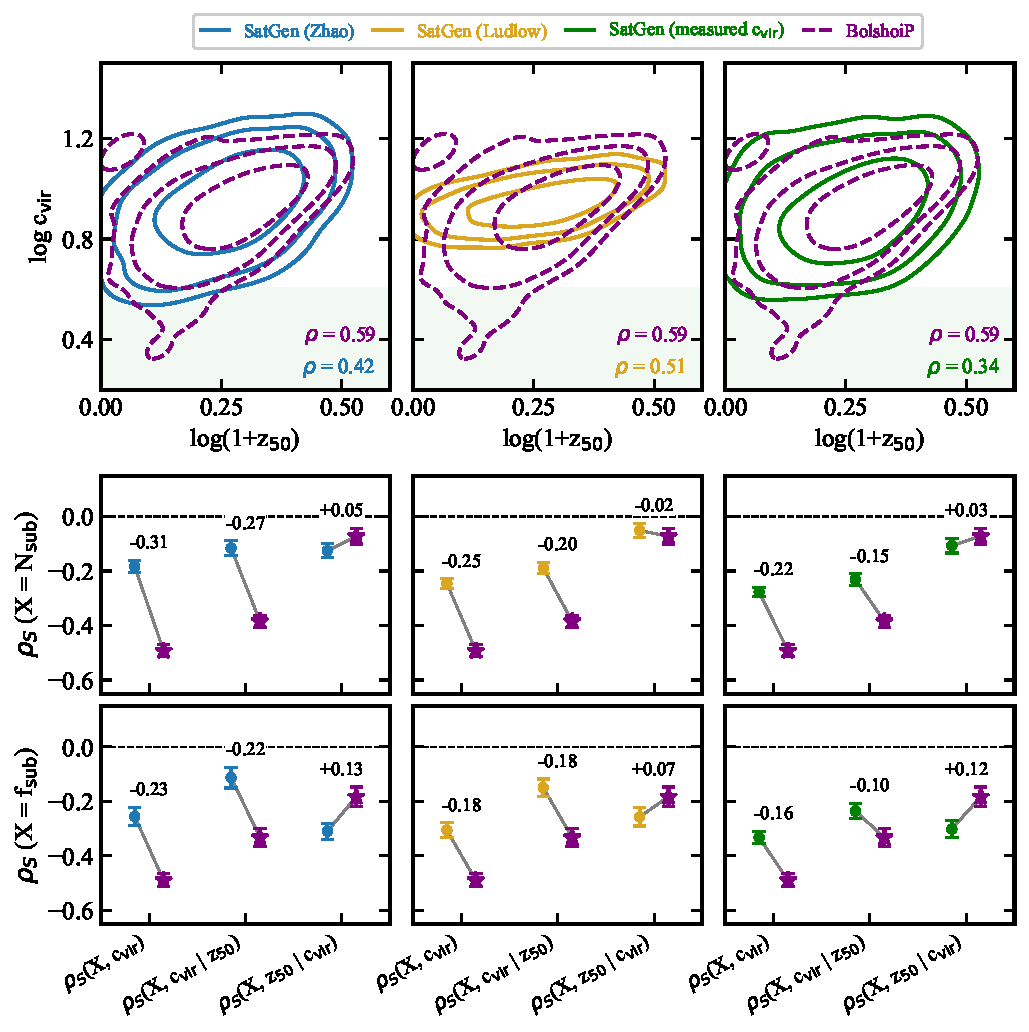
\includegraphics{figures/cvir_trends.pdf}
   \caption{\jsm{Concentration tests in the $\mathbb{S}_{13.2}$ sample. Each column compares the relaxed BolshoiP hosts (purple) with a version of the \SatGen\ model built from the same 1517 merger trees: the fiducial \cite{Zhao.etal.09} concentrations (blue), concentrations measured in the presence of substructure (green, Section \ref{sec:cvir_measurments}), and the \cite{Ludlow.etal.16} concentrations with subhalos re-evolved in the corresponding host potential (yellow, Section \ref{sec:ludlow}). Top row: the $\zfive \times \cvir$ distributions, with the $\rho_S(\zfive, \cvir)$ correlation coefficients in the bottom right corner of every panel. As in Figure \ref{fig:z50_cvir}, the light shaded region marks $\cvir < 4$. Middle and bottom rows: $\rho_S(X, \cvir)$, the concentration channel $\rho_S(X, \cvir \,|\, \zfive)$ and the formation-time channel $\rho_S(X, \zfive \,|\, \cvir)$ for $X = \nsub$ and $X = \fsub$, respectively. Each value of the \SatGen\ model is connected to its BolshoiP counterpart by a grey line, and the grey numbers give the difference $\Delta \rho_S$ between the two. Error bars are the jackknife uncertainties described in Section \ref{sec:correlation}.}}
   \label{fig:cvir_trends}
\end{figure*}

\section{Discussion}
\label{sec:discussion}

\subsection{Sequential versus Self-Consistent Assembly}
\label{sec:sequential}

Taken together, our results highlight the fundamental difference between the \SatGen\ model and the simulations in that our semi-analytic framework treats halo assembly and subhalo evolution as two sequential, largely isolated processes. In the first step of the model, merger trees are generated and the host halo concentrations are assigned according to the \cite{Zhao.etal.09} prescription. The resulting $\zfive$ and $\cvir$ distributions are therefore determined entirely by the adopted mapping between the MAH and halo concentration. In the second step of the model, the orbits of subhalos are evolved within their host halo's potentials which are defined by the first step. This means that subhalo populations can never alter or influence the mass assembly histories or concentrations of their hosts.

This separation is important because, in a cosmological simulation, these quantities are not independent inputs to one another. A halo's assembly history, internal structure, and subhalo population all emerge simultaneously from the same underlying dynamical process. These correlations provide multiple pathways through which halo assembly can influence the surviving subhalo population and visa-versa. This provides a natural explanation for why the assembly bias signals measured in the \SatGen\ model are generally weaker than those found in cosmological simulations.

\jsm{This separation also explains why varying the evolution of subhalos has little effect on the assembly bias signal. In Appendix \ref{sec:DF}, we show that increasing the strength of dynamical friction by a factor of five changes the normalization of the $\nsub$ and $\fsub$ distributions but leaves the rank-order correlations essentially unchanged, and in Appendix \ref{sec:threshold} we show the same for the choice of $\mthresh$. Both act on the evolution of subhalos within a fixed host potential, and hence on the formation-time channel, which the \SatGen\ model already reproduces. Neither can alter the host concentrations, where the discrepancy resides.}

\jsm{The isolation criterion applied in Section \ref{sec:fid} also provides the closest proxy for environment available in this comparison. As discussed in Section \ref{sec:intro}, EPS-based merger trees carry no information about the large-scale environment of a host, whereas in the simulations the tidal field of massive neighbors can stall the accretion of a halo and its subhalos \citep{Dalal.etal.08, Hahn.etal.09}. Because the relaxation and isolation criteria are applied together, we cannot separate their individual contributions. However, the discrepancy that remains after both cuts indicates that neither unrelaxed hosts nor hosts in dense environments fully account for the weaker assembly bias signals in the \SatGen\ model.}

\subsection{Inference on Mass Assembly Histories}
\label{sec:inference}

\jsm{need to cite Lucey et al}

Though the disparity at first might appear concerning, it is important to distinguish between the strength of a correlation and the ability to infer one quantity from another. Recently \cite{Monzon.etal.26} used random forest regression methods to demonstrate that a combination of present-day observables predicted by the \SatGen\ model can be used to infer metrics relevant to halo mass accretion histories. In short, they show that the combination of the stellar mass of the central galaxy ($M_{\rm cen}$), the accreted stellar halo ($M_{\rm ASH}$), and the cumulative mass of surviving satellites ($\Msat$) can be used to recover half-mass formation redshifts, the number of significant stellar-halo progenitors, and the accretion mass of the most massive progenitor. Lets assume that, in the context of $\Lambda$CDM, cosmological simulations are better suited than our semi-analytic framework for capturing the dynamic nature of structure formation. This implies that any signals of ``real'' assembly bias measured in observational data will be much stronger than what can be measured in our model (see Figure \ref{fig:correlations}). The results presented in \cite{Monzon.etal.26} are therefore even more encouraging because, despite its divided treatment of merger tree generation and subhalo evolution, the \SatGen\ model does produce useful connections between present-day satellite populations and halo assembly histories.

%\begin{figure}
%    \centering
%    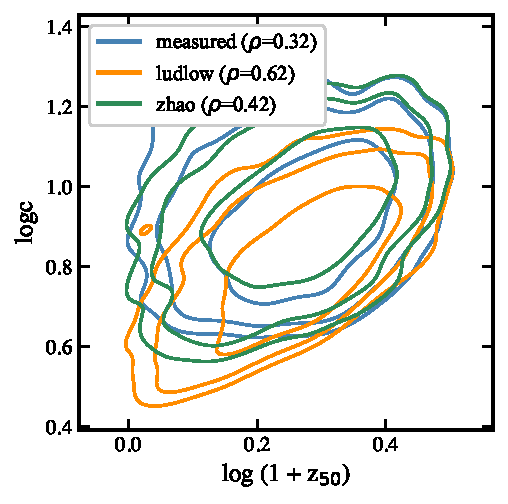
\includegraphics{figures/concentrations.pdf}
%    \caption{Caption}
%    \label{fig:placeholder}
%\end{figure}

%\begin{figure*}
%    \centering
%    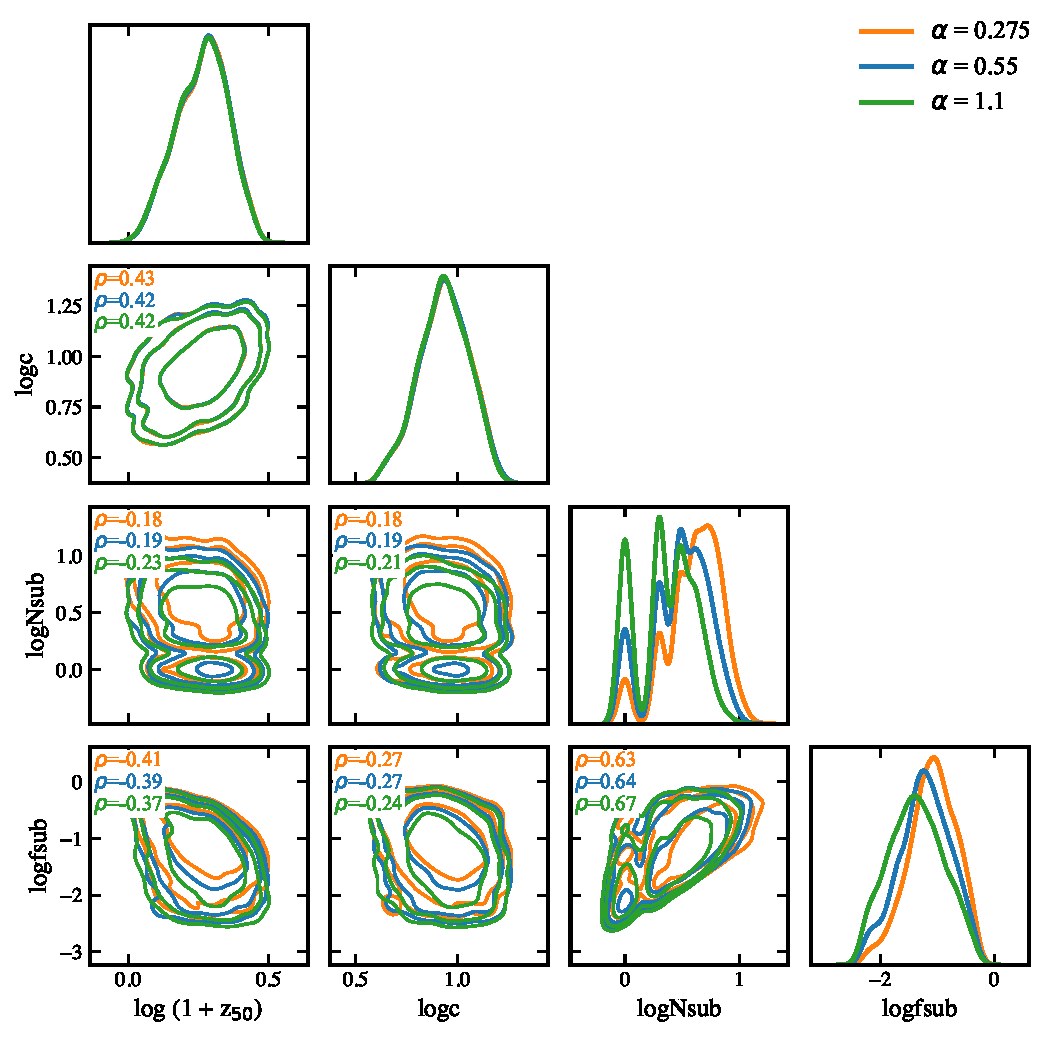
\includegraphics{figures/corner_alpha.pdf}
%    \caption{Caption}
%    \label{fig:placeholder}
%\end{figure*}

%\begin{figure*}
%    \centering
%    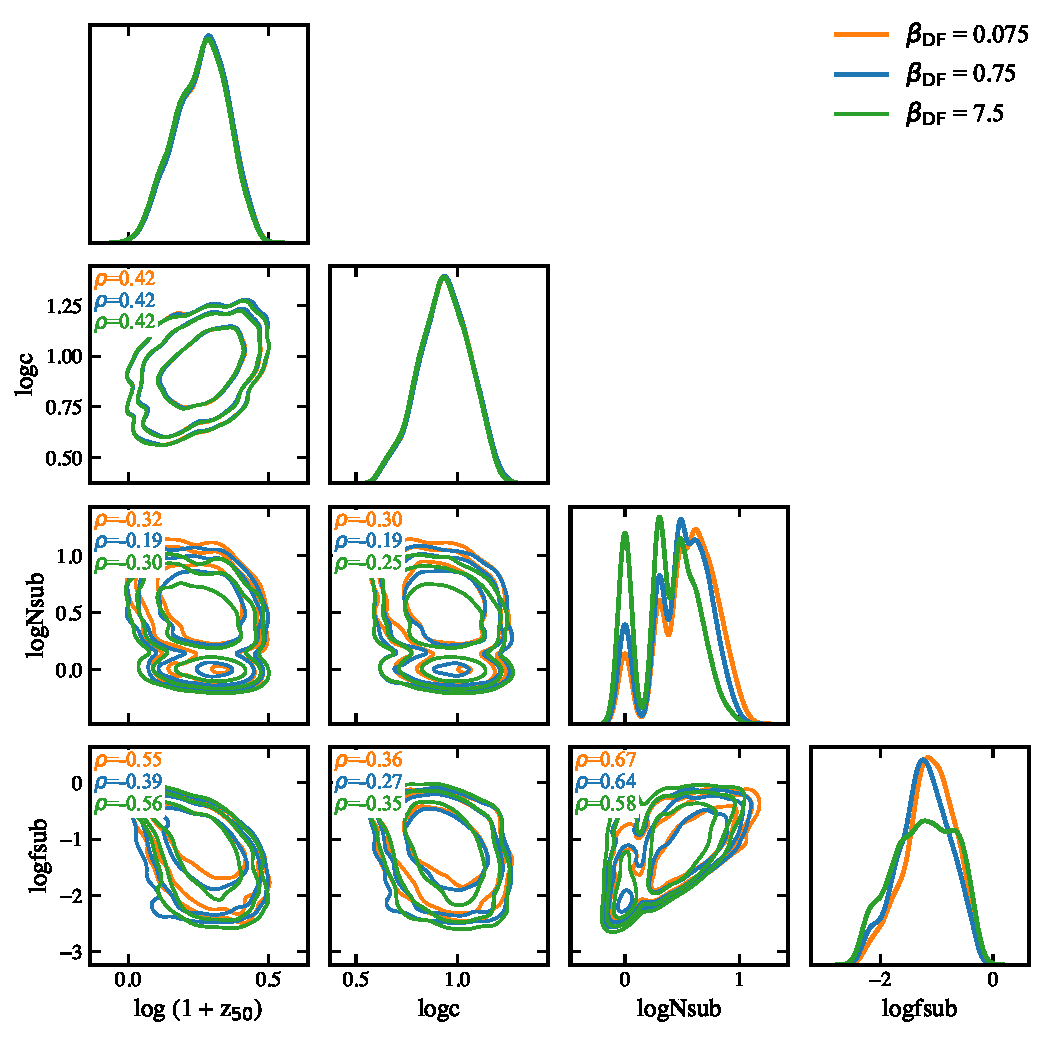
\includegraphics{figures/corner_beta.pdf}
%    \caption{Caption}
%    \label{fig:placeholder}
%\end{figure*}

\section{Summary and Conclusions}
\label{sec:conclusions}

This is an important step for \jsm{In forthcoming work, we extent this analysis by examining
whether such observables can be used to simultaneously infer
both halo mass and halo formation time.} and \jsm{In future work, we will use the model developed here to
examine stellar halos and satellite populations across a much wider range in host halo mass and investigate how their properties may inform characteristics of the SHMR, especially at the low-mass end.}

\section*{Acknowledgments}

The authors are grateful to \jsm{XXX} for valuable discussion, and to \jsm{XXX}. FvdB is supported by the National Science Foundation (NSF) through grant AST-2307280. This work was performed in part at the Kavli Institute for Theoretical Physics (KITP) in Santa Barbara, which is supported in part by the National Science Foundation under Grant No. NSF PHY-174895. The authors also acknowledge the Gauss Centre for Supercomputing e.V. (www.gauss-centre.eu) and the Partnership for Advanced Supercomputing in Europe (PRACE, www.prace-ri.eu) for funding the MultiDark simulation project by providing computing time on the GCS Supercomputer SuperMUC at Leibniz Supercomputing Centre (LRZ, www.lrz.de). The Bolshoi simulations have been performed within the Bolshoi project of the University of California High-Performance AstroComputing Center (UC-HiPACC) and were run at the NASA Ames Research Center.

This work made extensive use of the following python packages: \texttt{Matplotlib} \citep{Matplotlib_Hunter2007}, \texttt{SciPy} \citep{SciPy_Virtanen2020}, \texttt{NumPy} \citep{numpy_vanderWalt2011}, and \texttt{PyGTC} \citep{PyGTC_Bocquet2016}. 

\bibliographystyle{mnras}
%%\bibliographystyle{aasjournal}

\bibliography{references.bib}

\appendix

\subsection{Dynamical Friction}
\label{sec:DF}

\jsm{[moved here from obsolete.tex]}

\begin{figure*}
    \centering
     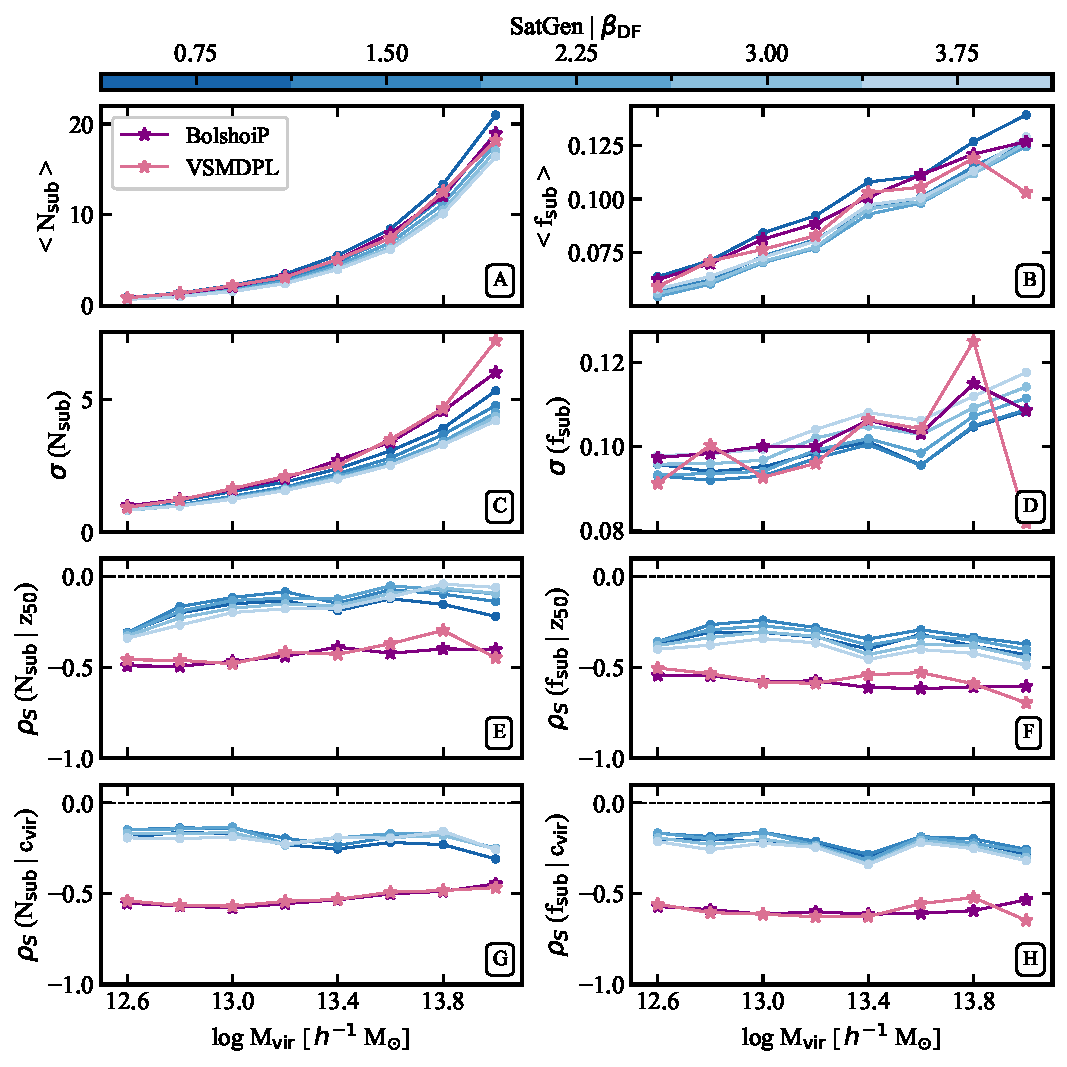
\includegraphics{figures/DF_full.pdf}
    \caption{The assembly bias signal of the \SatGen\ model as a function of the strength of dynamical friction. Here the BolshoiP simulation is shown in purple and VSMDPL in pink but now the \SatGen\ model is colored by the assumed value of $\betadf$ as indicated. Our fiducial model $\betadf = 0.75$ corresponds to the darkest shade of blue, while the lightest shade corresponds to a 5x increase in the assumed strength of dynamical friction. The means of the $<\nsub>$ and $<\fsub>$ distributions (per host halo mass sample), are shown in Panels A and B, respectively. Similarly, the standard deviations of the $\sigma(\nsub)$ and $\sigma(\fsub)$ distributions, are shown in Panels C and D, respectively. We show the same correlation coefficients as in Figure \ref{fig:correlations} with $\rho_S(\nsub, \zfive)$ in panel E, $\rho_S(\fsub, \zfive)$ in panel F, $\rho_S(\nsub, \cvir)$ in panel G, and finally $\rho_S(\fsub, \cvir)$ in panel H. For clarity, the jack-knife errorbars were not plotted but are qualitatively the same as before. Notice that though $\betadf$ impacts the top four panels, it does not significantly change the measured assembly bias signal in the bottom four panels.}
    \label{fig:DF}
\end{figure*}

In this section we discuss one of the main parameters that governs the mass loss of subhalos in our semi-analytic framework and which can in principal be tuned to match simulations: the strength of dynamical friction. In the \SatGen\ model each subhalo is integrated in the potential of its direct parent, accounting for a dynamical friction force
%
\begin{equation}
F_{\rm DF}=-4 \pi \frac{G^2 m^2 }{v^2} \, \log{\Lambda} \, \rho(<v) \, \frac{v}{| v | } 
\end{equation}
%
\citep{Chandrasekhar.43}. Here, $m$ is the instantaneous subhalo mass, $\log \Lambda$ is the Coulomb logarithm, $v$ is the relative velocity of the subhalo with respect to its parent halo, and $\rho(<v)$ is the local density of dark matter particles in the parent halo with a speed less than $|v|$, which is computed under the standard assumption that the particles follow an isotropic Maxwellian velocity distribution \citep[see][]{Binney.Tremaine.08}. The Coulomb logarithm is modeled using
%
\begin{equation}\label{coulomb}
\log \Lambda= \betadf \, \log \left(M / m\right)\,,
\end{equation}
%
where $M$ is the instantaneous mass of the parent halo and $\beta_{\rm DF}$ is a free parameter that regulates the overall strength of dynamical friction. For comparisons to BolshoiP, \cite{Green.etal.21} found that $\beta_{\rm DF} = 0.75$ worked best at reproducing present-day radial distributions. \cite{Monzon.etal.26} instead adopted a fiducial value of $\beta_{\rm DF} = 1.0$ and showed how varying this parameter by a factor 2 does not significantly impact the \SatGen\ model's prediction for the accreted stellar halos around MW-like galaxies.

To investigate the impact of $\betadf$ on the assembly bias signal, we took the 8,000 trees described in Section \old{{\ref{sec:DF}}} \jsm{\ref{sec:satgen}} and reran our model's orbit integration step four more times, resulting in a set of five models with $\beta_{\rm DF} = [0.75, 1.5, 2.25, 3.00, 3.75]$. Because we reused the same merger trees, each host has identical $\zfive$ and $\cvir$ values across all five models. This means that changing $\betadf$ can alter the assembly bias signal only if its effect on the subhalo populations depends systematically on host assembly history—for example, if it preferentially modifies the subhalo populations of a subset of hosts within a given mass bin. We show the results of this test in Figure \ref{fig:DF} as a function of $\Mvir$.

As before, BolshoiP is shown in purple and VSMDPL in pink. Now the \SatGen\ model is colored by the assumed value of $\betadf$ as indicated. The means, $<\nsub>$ and $<\fsub>$, are shown in Panels A and B, respectively. Similarly, the standard deviations, $\sigma(\nsub)$ and $\sigma(\fsub)$, are shown in Panels C and D, respectively. The bottom four panels show the same rank-order correlation coefficients as in Figure \ref{fig:correlations}, but this time for each of the $\betadf$ models. Specifically, we show $\rho_S(\nsub, \zfive)$ in panel E, $\rho_S(\fsub, \zfive)$ in panel F, $\rho_S(\nsub, \cvir)$ in panel G, and finally $\rho_S(\fsub, \cvir)$ in panel H. 

The clear color gradients in Panels A and B show that, as expected, increasing $\betadf$ results in fewer, less massive subhalos. We can also see that, in terms of $<\nsub>$ and $<\fsub>$, our fiducial value of $\betadf$ is in good agreement with the MultiDark suite. The standard deviations $\sigma(\nsub)$ and $\sigma(\fsub)$ in Panels C and D show that our fiducial model slightly underpredicts the width of the distributions for higher values of $\Mvir$ and that increasing $\betadf$ has the opposite effect on $\sigma(\nsub)$ than it does on $\sigma(\fsub)$. This differing response is not necessarily unexpected, since $\nsub$ can be nicely approximated as a Poisson distribution \citep{Jiang.vdBosch.17}, but $\fsub$ depends not only on the number of surviving subhalos but also on their individual masses and correlations between their masses. Finally, the lack of clear color gradients in Panels E, F, G, and H shows that tuning this free parameter does not significantly impact the \SatGen\ model's assembly bias signal.

Because dynamical friction primarily impacts the orbits of systems with high merger ratios \citep{vdBosch.99}, only a subset of the overall subhalo population is strongly affected by changes in $\betadf$. Consequently, while changing $\betadf$ could produce a substantial effect on these hosts, its impact on the entire population is diluted by the larger fraction of hosts whose subhalo populations are largely insensitive to $\betadf$. In other words, while increasing $\betadf$ systematically shifts the normalization of $\nsub$ and $\fsub$ across the entire population, it does not significantly reshape the subhalo populations of hosts as a function of their particular assembly history.

Though $\betadf$ primarily controls the efficiency with which a subhalo's orbit decays and can shift the normalization of the surviving subhalo population, within our semi-analytic framework, it is not itself a significant driver of the assembly bias signal. This result is perhaps not unsurprising given that, in this experiment, varying $\betadf$ does not directly impact either the $\zfive$ or $\cvir$ distributions. This is because both distributions are set in the initial merger tree generation step and not in the subsequent orbit evolution step\footnote{Introducing a coupling between concentration, mass accretion histories, and our analytic prescription for dynamical friction would likely require iterating across both the merger tree generation and orbit evolution steps. This would introduce substantial computational overhead relative to our current pipeline and would require an empirically-derived convergence limit.}. Thus, this experiment tests whether changing orbital evolution at fixed assembly history can generate an additional assembly bias signal. The bottom four panels show that even a factor of 5 in the assumed value of $\betadf$ produces little change in the rank-order correlations between the surviving subhalo populations and either $\zfive$ or $\cvir$.


\subsection{Minimum Mass Threshold}
\label{sec:threshold}

As described in \ref{sec:counts}, both $\nsub$ and $\fsub$ are defined according to $\mthresh = 7.75 \times 10^{10} \Msunh$. This fiducial value was chosen by the 500 particle mass resolution limit in BolshoiP but can arbitrarily be varied. Of course the main consideration is that subhalo properties become less reliable the further down $\mthresh$ is assumed to be. In the case of \texttt{ROCKSTAR} analysis of the MultiDark suite, \cite{RodriguezPuebla.etal.16} claim they can reliably identify subhalos with $\gtrsim 100$ particles. This is consistent with \cite{Klypin.etal.16} who argue that while $\gtrsim 250$ particles is required to faithfully resolve the innermost regions of these systems, but that one can estimate key properties such as subhalo mass and virial radius with fewer than $250$ particles.

To further investigate the impact of numerical resolution on our comparison, we recalculated $\nsub$ and $\fsub$ for $\mthresh = 7.75 \times 10^{9} \Msunh$ and $\mthresh = 1.5 \times 10^{11} \Msunh$ and remeasured the assembly bias signal for all three models. As before in Section \ref{sec:DF}, we do not vary either the $\zfive$ or $\cvir$ distributions. We are therefore testing if the effect of changing $\mthresh$ depends systematically on host halo assembly. The results of this test are shown in Figure \ref{fig:massthresh} where once again, the \SatGen\ model is shown in blue, BolshoiP is shown in purple and VSMDPL in pink. Just as in Figure \ref{fig:correlations}, we show $\rho_S(\nsub, \zfive)$ in panel A, $\rho_S(\fsub, \zfive)$ in panel B, $\rho_S(\nsub, \cvir)$ in panel C, and finally $\rho_S(\fsub, \cvir)$ in panel D. Here, the different lifestyles indicate which minimum mass threshold was to measure the assembly bias signal. For clarity, we show the $\mthresh = 7.75 \times 10^{9} \Msunh$ model (50 particles in BolshoiP and 1,250 in VSMDPL) as the solid lines to indicate the ``highest'' resolution measurements. For clarity we have once again omitted the error bars but they remain qualitatively the same.

Figure \ref{fig:massthresh} clearly shows that the measured assembly bias signals are not strongly sensitive to $\mthresh$. In fact, across all three models, the largest differences in correlation strengths are observed when the assembly bias signal is measured with respect to $\nsub$ as opposed to $\fsub$. This makes sense since, if one considers the results shown in Figure \ref{fig:SHMF}, for which $\rm{d}N / \rm{d}\log(m/M) \propto (m/M)^{-0.88}$ such that the number of subhalos is strongly weighted towards the low-mass end of the SHMF. This means that increasing $\mthresh$ can have a noticeable impact on $\nsub$ but has a much smaller effect on $\fsub$, for which the contribution of each subhalo is weighted by its mass. 

Across all four metrics, changing from $\mthresh = 7.75 \times 10^{9} \Msunh$ to $\mthresh = 1.5 \times 10^{11} \Msunh$ only results in $\Delta \rho \lesssim 0.1$ for the simulations and $\Delta \rho \lesssim 0.2$ in the \SatGen\ model. This is interesting given that, for BolshoiP, $\mthresh = 7.75 \times 10^{9} \Msunh$ no longer satisfies the $\sim 100$ particle criteria. This indicates that the assembly bias signal measured in DMO simulations is robust against halo finder uncertainties introduced by finite mass resolution. This is consistent with the fact that, despite VSMDPL achieving a much higher mass resolution than BolshoiP, their measured assembly bias signals are almost identical (see also Figure \ref{fig:correlations}).

In summary, though $\mthresh$ effectively sets $\nsub$, it is not itself a significant driver of the assembly bias signal. Again, because both the $\zfive$ and $\cvir$ distributions are set in the initial merger tree generation step, this experiment tests whether changing the minimum mass threshold at fixed assembly history can generate an additional assembly bias signal. We show that increasing the mass resolution of in the simulations by a factor of $\sim 20$ does not significantly alter the rank-order correlations between the surviving subhalo populations and either $\zfive$ or $\cvir$.

%\begin{figure*}
%    \centering
%     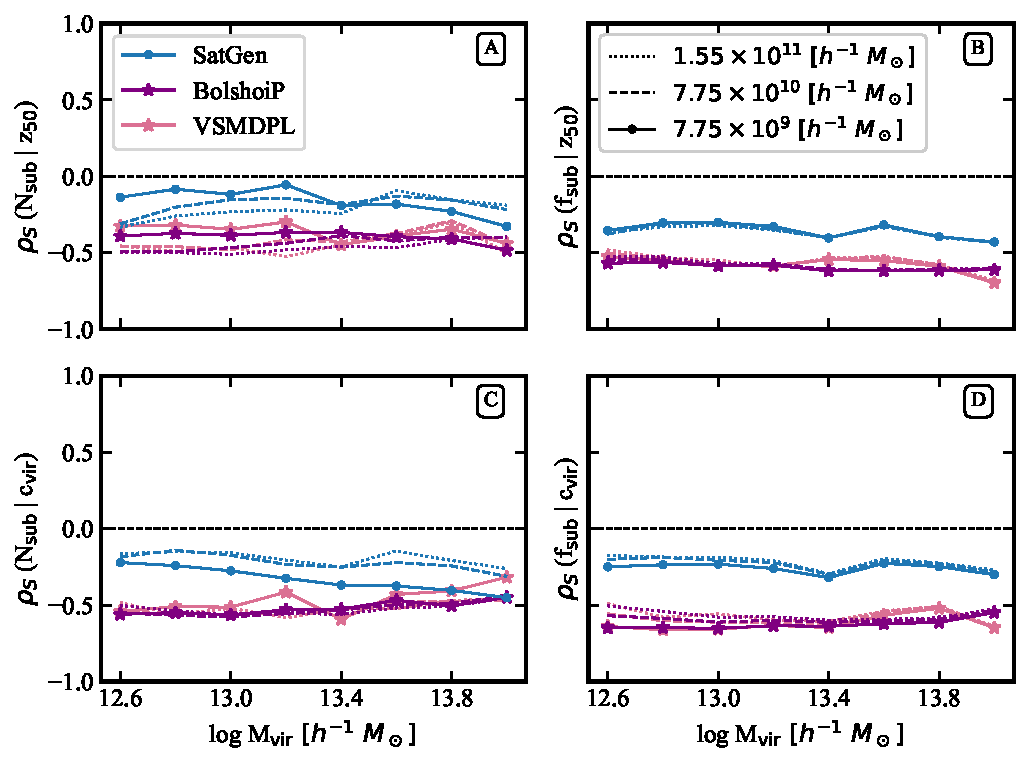
\includegraphics{figures/mass_thresfull.pdf}
%    \caption{The effect of varying the minimum mass threshold $\mthresh$ on the assembly bias signals. As before, the three models are distinguished by color as indicated by the legend. Just as in Figure \ref{fig:correlations}, we show $\rho_S(\nsub, \zfive)$ in panel A, $\rho_S(\fsub, \zfive)$ in panel B, $\rho_S(\nsub, \cvir)$ in panel C, and finally $\rho_S(\fsub, \cvir)$ in panel D. Here the different lifestyles correspond to the different values assumed for $\mthresh$ as indicated. For reference, the three thresholds shown correspond to 1000 (dotted), 500 (dashed) and 50 (solid) particles in BolshoiP. Once again, the jack-knife errorbars were not plotted but are qualitatively the same as before.}
%    \label{fig:massthresh}
%\end{figure*}

\jsm{Discuss \cite{Nadler.etal.23b} and \cite{Zentner.07} who both use minimum mass thresholds relative to the host, \cite{Zentner.07} in particular shows what happens what happens to the correlation between z50 and Nsat when the threshold decreases but they do so in a narrow range where 0.1 < Vsat/Vhost < 0.5. In our highest mass range we range from have -4 < log(msat/Mhost) < -3 and in our lowest mass range we have -3 < log(msat/Mhost) < -2.}




\end{document}


